% Created 2024-05-29 Wed 17:58
% Intended LaTeX compiler: pdflatex
\documentclass[a4paper]{article}
                      \usepackage[utf8]{inputenc}
\usepackage{amsmath, amssymb, amsfonts, amsthm,multirow}
\usepackage{geometry}
\geometry{margin=2cm}
\usepackage[colorlinks=true, linktoc=all, linkcolor=black, citecolor=red, urlcolor=blue]{hyperref}
\numberwithin{equation}{section}
\setcounter{secnumdepth}{2}
\setcounter{tocdepth}{2}
\usepackage{listings}
\setcounter{secnumdepth}{2}
\author{Paul ROUX}
\date{\today}
\title{JuliVirBootstrap Documentation}
\hypersetup{
 pdfauthor={Paul ROUX},
 pdftitle={JuliVirBootstrap Documentation},
 pdfkeywords={},
 pdfsubject={},
 pdfcreator={Emacs 29.1 (Org mode 9.7)}, 
 pdflang={English}}

% Setup for code blocks [1/2]

\usepackage{fvextra}

\fvset{%
  commandchars=\\\{\},
  highlightcolor=white!95!black!80!blue,
  breaklines=true,
  breaksymbol=\color{white!60!black}\tiny\ensuremath{\hookrightarrow}}

% Make line numbers smaller and grey.
\renewcommand\theFancyVerbLine{\footnotesize\color{black!40!white}\arabic{FancyVerbLine}}

\usepackage{xcolor}

% In case engrave-faces-latex-gen-preamble has not been run.
\providecolor{EfD}{HTML}{f7f7f7}
\providecolor{EFD}{HTML}{28292e}

% Define a Code environment to prettily wrap the fontified code.
\usepackage[breakable,xparse]{tcolorbox}
\DeclareTColorBox[]{Code}{o}%
{colback=EfD!98!EFD, colframe=EfD!95!EFD,
  fontupper=\footnotesize\setlength{\fboxsep}{0pt},
  colupper=EFD,
  IfNoValueTF={#1}%
  {boxsep=2pt, arc=2.5pt, outer arc=2.5pt,
    boxrule=0.5pt, left=2pt}%
  {boxsep=2.5pt, arc=0pt, outer arc=0pt,
    boxrule=0pt, leftrule=1.5pt, left=0.5pt},
  right=2pt, top=1pt, bottom=0.5pt,
  breakable}

% Support listings with captions
\usepackage{float}
\floatstyle{plain}
\newfloat{listing}{htbp}{lst}
\newcommand{\listingsname}{Listing}
\floatname{listing}{\listingsname}
\newcommand{\listoflistingsname}{List of Listings}
\providecommand{\listoflistings}{\listof{listing}{\listoflistingsname}}


% Setup for code blocks [2/2]: syntax highlighting colors

\newcommand\efstrut{\vrule height 2.1ex depth 0.8ex width 0pt}
\definecolor{EFD}{HTML}{000000}
\definecolor{EfD}{HTML}{ffffff}
\newcommand{\EFD}[1]{\textcolor{EFD}{#1}} % default
\definecolor{EFvp}{HTML}{000000}
\newcommand{\EFvp}[1]{\textcolor{EFvp}{#1}} % variable-pitch
\definecolor{EFh}{HTML}{7f7f7f}
\newcommand{\EFh}[1]{\textcolor{EFh}{#1}} % shadow
\definecolor{EFsc}{HTML}{228b22}
\newcommand{\EFsc}[1]{\textcolor{EFsc}{\textbf{#1}}} % success
\definecolor{EFw}{HTML}{ff8e00}
\newcommand{\EFw}[1]{\textcolor{EFw}{\textbf{#1}}} % warning
\definecolor{EFe}{HTML}{ff0000}
\newcommand{\EFe}[1]{\textcolor{EFe}{\textbf{#1}}} % error
\definecolor{EFl}{HTML}{ff0000}
\newcommand{\EFl}[1]{\textcolor{EFl}{#1}} % link
\definecolor{EFlv}{HTML}{ff0000}
\newcommand{\EFlv}[1]{\textcolor{EFlv}{#1}} % link-visited
\definecolor{EFhi}{HTML}{ff0000}
\newcommand{\EFhi}[1]{\textcolor{EFhi}{#1}} % highlight
\definecolor{EFc}{HTML}{b22222}
\newcommand{\EFc}[1]{\textcolor{EFc}{#1}} % font-lock-comment-face
\definecolor{EFcd}{HTML}{b22222}
\newcommand{\EFcd}[1]{\textcolor{EFcd}{#1}} % font-lock-comment-delimiter-face
\definecolor{EFs}{HTML}{8b2252}
\newcommand{\EFs}[1]{\textcolor{EFs}{#1}} % font-lock-string-face
\definecolor{EFd}{HTML}{8b2252}
\newcommand{\EFd}[1]{\textcolor{EFd}{#1}} % font-lock-doc-face
\definecolor{EFm}{HTML}{008b8b}
\newcommand{\EFm}[1]{\textcolor{EFm}{#1}} % font-lock-doc-markup-face
\definecolor{EFk}{HTML}{9370db}
\newcommand{\EFk}[1]{\textcolor{EFk}{#1}} % font-lock-keyword-face
\definecolor{EFb}{HTML}{483d8b}
\newcommand{\EFb}[1]{\textcolor{EFb}{#1}} % font-lock-builtin-face
\definecolor{EFf}{HTML}{0000ff}
\newcommand{\EFf}[1]{\textcolor{EFf}{#1}} % font-lock-function-name-face
\definecolor{EFv}{HTML}{a0522d}
\newcommand{\EFv}[1]{\textcolor{EFv}{#1}} % font-lock-variable-name-face
\definecolor{EFt}{HTML}{228b22}
\newcommand{\EFt}[1]{\textcolor{EFt}{#1}} % font-lock-type-face
\definecolor{EFo}{HTML}{008b8b}
\newcommand{\EFo}[1]{\textcolor{EFo}{#1}} % font-lock-constant-face
\definecolor{EFwr}{HTML}{ff0000}
\newcommand{\EFwr}[1]{\textcolor{EFwr}{\textbf{#1}}} % font-lock-warning-face
\newcommand{\EFnc}[1]{#1} % font-lock-negation-char-face
\definecolor{EFpp}{HTML}{483d8b}
\newcommand{\EFpp}[1]{\textcolor{EFpp}{#1}} % font-lock-preprocessor-face
\newcommand{\EFrc}[1]{\textbf{#1}} % font-lock-regexp-grouping-construct
\newcommand{\EFrb}[1]{\textbf{#1}} % font-lock-regexp-grouping-backslash
\newcommand{\EFob}[1]{#1} % org-block
\newcommand{\EFobb}[1]{#1} % org-block-begin-line
\newcommand{\EFobe}[1]{#1} % org-block-end-line
\definecolor{EFOa}{HTML}{0000ff}
\newcommand{\EFOa}[1]{\textcolor{EFOa}{#1}} % outline-1
\definecolor{EFOb}{HTML}{a0522d}
\newcommand{\EFOb}[1]{\textcolor{EFOb}{#1}} % outline-2
\definecolor{EFOc}{HTML}{a020f0}
\newcommand{\EFOc}[1]{\textcolor{EFOc}{#1}} % outline-3
\definecolor{EFOd}{HTML}{b22222}
\newcommand{\EFOd}[1]{\textcolor{EFOd}{#1}} % outline-4
\definecolor{EFOe}{HTML}{228b22}
\newcommand{\EFOe}[1]{\textcolor{EFOe}{#1}} % outline-5
\definecolor{EFOf}{HTML}{008b8b}
\newcommand{\EFOf}[1]{\textcolor{EFOf}{#1}} % outline-6
\definecolor{EFOg}{HTML}{483d8b}
\newcommand{\EFOg}[1]{\textcolor{EFOg}{#1}} % outline-7
\definecolor{EFOh}{HTML}{8b2252}
\newcommand{\EFOh}[1]{\textcolor{EFOh}{#1}} % outline-8
\definecolor{EFhn}{HTML}{008b8b}
\newcommand{\EFhn}[1]{\textcolor{EFhn}{#1}} % highlight-numbers-number
\definecolor{EFhq}{HTML}{9370db}
\newcommand{\EFhq}[1]{\textcolor{EFhq}{#1}} % highlight-quoted-quote
\definecolor{EFhs}{HTML}{008b8b}
\newcommand{\EFhs}[1]{\textcolor{EFhs}{#1}} % highlight-quoted-symbol
\definecolor{EFrda}{HTML}{707183}
\newcommand{\EFrda}[1]{\textcolor{EFrda}{#1}} % rainbow-delimiters-depth-1-face
\definecolor{EFrdb}{HTML}{7388d6}
\newcommand{\EFrdb}[1]{\textcolor{EFrdb}{#1}} % rainbow-delimiters-depth-2-face
\definecolor{EFrdc}{HTML}{909183}
\newcommand{\EFrdc}[1]{\textcolor{EFrdc}{#1}} % rainbow-delimiters-depth-3-face
\definecolor{EFrdd}{HTML}{709870}
\newcommand{\EFrdd}[1]{\textcolor{EFrdd}{#1}} % rainbow-delimiters-depth-4-face
\definecolor{EFrde}{HTML}{907373}
\newcommand{\EFrde}[1]{\textcolor{EFrde}{#1}} % rainbow-delimiters-depth-5-face
\definecolor{EFrdf}{HTML}{6276ba}
\newcommand{\EFrdf}[1]{\textcolor{EFrdf}{#1}} % rainbow-delimiters-depth-6-face
\definecolor{EFrdg}{HTML}{858580}
\newcommand{\EFrdg}[1]{\textcolor{EFrdg}{#1}} % rainbow-delimiters-depth-7-face
\definecolor{EFrdh}{HTML}{80a880}
\newcommand{\EFrdh}[1]{\textcolor{EFrdh}{#1}} % rainbow-delimiters-depth-8-face
\definecolor{EFrdi}{HTML}{887070}
\newcommand{\EFrdi}[1]{\textcolor{EFrdi}{#1}} % rainbow-delimiters-depth-9-face
\usepackage{biblatex}

\begin{document}

\maketitle
\setcounter{tocdepth}{3}
\tableofcontents

\section{Overview}
\label{sec:org222ff30}

This document contains a program for performing conformal bootstrap computations in 2D loop models.

The program relies on the assumption that the spectrum of the model contains degenerate fields \(V^d_{\langle1,s\rangle}\) (see below).
\begin{itemize}
\item TODO: remember to cite \href{https://arxiv.org/abs/2105.03949}{arXiv:2105.03949} for Julia Symbolics
\label{sec:org996118c}
\end{itemize}
\section{Conformal bootstrap in 2D}
\label{sec:org91b71e5}

\subsection{Notations, parametrisations}
\label{sec:org75571db}

\subsubsection*{Central charge}
\label{sec:org64ec19c}

We parametrise the central charge of our theories in terms of variables \(B\), \(b\) or \(\beta\) related by

\[c = 13 + 6B + 6 B^{-1} \quad , \quad B = b^2 = -\beta^2, \quad B = \frac{c-13 \pm \sqrt{(c-1)(c-25)}}{12}\]

By convention we keep
\subsubsection*{Fields}
\label{sec:org6f0e859}

We parametrise the conformal dimensions \((\Delta, \bar\Delta)\) of fields in terms of variables \(P, p, \delta\), related by

\[
\Delta = \frac{c-1}{24} + \delta  \quad , \quad \delta = P^2 = -p^2
\]

The variable \(P\) is called the momentum. By convention, we always keep \(P=ip\).Moreover, we introduce the following parametrisation of dimensions in terms of Kac indices \(r, s\):

\[P_{(r,s)}=\frac{1}{2}(\beta r - \beta^{-1}s)\]

where \(r,s\) are arbitrary numbers. We say the field is degenerate if \(r,s\in \mathbb Z\) and \(rs > 0\).
This convention is different from the one in \href{https://gitlab.com/s.g.ribault/Bootstrap\_Virasoro.git}{Sylvain's code}, but similar to our more recent conventions, such as in \href{https://github.com/ribault/CFT-Review}{Sylvain's review on solvable CFTs}.

In loop models, we denote \(V_{(r,s)}\) a non-diagonal field of left and right momenta \((P_{(r,s)},P_{(r,-s)})\).
\subsection{Special functions}
\label{sec:org8205ee0}

Expressions of correlation functions in CFT involve special functions. In this paragraph we introduce some representations and regularisations of special functions.
\subsubsection*{Digamma function}
\label{sec:orgfd503a6}

The digamma function is defined for as

\begin{align}
  \psi(z) = \frac{\Gamma'(z)}{\Gamma(z)}
\end{align}

The function \(\psi\) has poles at negative integers. We regularise the digamma function thanks to the equation

\begin{align}
  \psi(1-x) - \psi(x) = \pi \operatorname{cot}(\pi x)
\end{align}

which means we use the regularization

\begin{align}
  \psi(-r) \underset{r\in\mathbb{N}}{=} \psi(r+1)
\end{align}
\subsubsection*{Barne's G-function and the double Gamma function}
\label{sec:org173abc3}

We need to compute the double Gamma function defined by the relations

\begin{align}
 \Gamma_{\beta}= \Gamma_{\beta^{-1}}, \quad, \Gamma_{\beta}\left( \frac{\beta + \beta^{-1}}{2} \right) = 1, \quad \Gamma_{\beta}(w + \beta) = \sqrt{2\pi} \frac{\beta^{\beta w-\frac{1}{2}}}{\Gamma(\beta w)} \Gamma_{\beta}(w)
\end{align}

(see \href{https://en.wikipedia.org/wiki/Multiple\_gamma\_function}{wikipedia article}).

It also obeys

\begin{align}
  \Gamma_{\beta}(w+\beta^{-1}) = \sqrt{2\pi} \frac{\beta^{-\beta^{-1}w+\frac12}}{\Gamma(\beta^{-1}w)} \Gamma_{\beta}(w).
\end{align}

For computing \(\Gamma_\beta\) it is convenient to use its relation to the Barne's \(G\) -function (see \href{https://en.wikipedia.org/wiki/Barnes\_G-function}{wikipedia article}), which is related to \(\Gamma_\beta\) as

\begin{align}
\Gamma_\beta(w) = \frac{\Gamma_2(w|\beta,\beta^{-1})}{\Gamma_2\left(\frac{\beta+\beta^{-1}}{2}\middle|\beta,\beta^{-1}\right)} \quad , \quad
 \Gamma_2(w|\beta,\beta^{-1})=(2\pi)^{\frac{w}{2\beta}} \beta^{\frac{w}{2}(w-\beta-\beta^{-1})+1} G(\beta^{-1}w,\beta^{-2})^{-1}
\end{align}

According to the theorem 1 in \href{https://arxiv.org/abs/2208.13876}{arXiv:2208.13876}, the \(G\) function has the following product representation

\begin{align}
  G(z, \tau) = G_{N}(z, \tau) \exp\left(z^{3} R_{M,N}(z,\tau) + O(N^{-M-1})\right)
\end{align}

where \(G_N\) is defined in terms of Gamma and polygamma functions,

\begin{align}\label{eq:Barnes_{GN}}
 G_N(z,\tau) = \frac{1}{\tau\Gamma(z)} e^{a(\tau) \frac{z}{\tau}+b(\tau)\frac{z^2}{2\tau^2}}
 \prod_{m=1}^N \frac{\Gamma(m\tau)}{\Gamma(z+m\tau)}e^{z\psi(m\tau)+\frac{z^2}{2}\psi'(m\tau)}
\end{align}

while \(R_{M, N}\) is a linear combination of certain polynomials \(P_k\),

\begin{align}
R_{M, N}(z,\tau) = \sum_{k=1}^M (k-1)!(-\tau)^{-k-1}P_k(z, -\tau) N^{-k}
\end{align}

where the polynomials are defined recursively by \(P_1(z,\tau)=\frac16\), and

\begin{align}
P_n(z,\tau) = \frac{z^{n-1}}{(n+2)!}-\frac{1}{\tau}\sum_{k=1}^{n-1} \frac{(1+\tau)^{k+2}-1-\tau^{k+2}}{(k+2)!} P_{n-k}(z,\tau)
\end{align}

It remains to define the coefficients

\begin{align}
a(\tau) = \tfrac12\tau\log(2\pi\tau) +\tfrac12\log(\tau) -\tau C(\tau) \quad , \quad b(\tau) =-\tau\log(\tau) -\tau^2D(\tau)
\end{align}

where the modular forms \(C(\tau),D(\tau)\) are

\begin{align}\label{eq:modular_C}
C(\tau) &= \frac{1}{2\tau}\log(2\pi) -\int_0^\infty dx\left[ \frac{e^{(1-\tau)x}}{2\sinh(x)\sinh(\tau x)}- \frac{e^{-2x}}{\tau x}\left(\frac{e^{x}}{2\sinh(x)}+1-\frac{\tau}{2}\right)\right]
\\
\label{eq:modular_D}
D(\tau) &= \int_0^\infty dx\left[ \frac{x e^{(1-\tau)x}}{\sinh(x)\sinh(\tau x)} - \frac{e^{-2x}}{\tau x}\right]
\end{align}

(We rewrite denominators in terms of \(\sinh\) in order to minimize numerical errors.)

For numerical evaluation of these integrals, it is useful to know the expansion of their integrands as \(x\to 0\):

\begin{align}
C(x, \tau) = \frac{2}{\tau} - \frac32 + \frac{\tau}{6} + \left(\frac56 - \frac{2}{\tau} + \frac{\tau}{6}\right)x  + \left( \frac4{3\tau} - \frac23 + \frac1{18}\tau - \frac{1}{90}\tau^{3}\right) x^{2}\quad , \quad D_0 = \frac{3}{\tau}-1
\end{align}

The error is of order \(\left(\frac{eN}{M}\right)^{-M}\), and the computation time of order \(N+ M^2\). To minimize computation time while keeping the error of order \(10^{-d}\), we take values of the type

\begin{align}
N = 20M, \quad M = \frac{\log(10)}{\alpha\log(20)}d
\end{align}

where \(\alpha\) is a parameter for reducing \(M\), which otherwise is too high in practice.
Up to logarithmic factors, the computation time is of order \(d^2\), whereas it should be of order \(d\) for the integral formula.
\subsection{Four point functions on the sphere}
\label{sec:orgd9af94c}

\subsubsection*{Chiral and non chiral blocks}
\label{sec:orgc75b474}

Because of conformal invariance, computation of any four-point correlation function on the sphere reduces to the computation of

$$ \mathcal G(x) = \langle V_{1}(x) V_{2}(0) V_{3}(\infty) V_{4}(1) \rangle $$

Four-point correlation functions can be written in terms of Virasoro blocks as

\begin{align}
  \mathcal G(x) = \sum_{k \in \mathcal S} \frac{C_{12k} C_{k34}}{B_{k}} \mathcal G_{\Delta_k}^{(s)}(c |\Delta_{1}, \dots, \Delta_{4}|z)\end{align}

We call \(\mathcal G_{\Delta_k}^{(s)}(c |\Delta_{1}, \dots, \Delta_{4}|z)\) a non-chiral conformal block.
In the case of a non-logarithmic theory, conformal blocks factorise as

\begin{align}
  \mathcal G_{\Delta_k}^{(s)}(c |\Delta_{1}, \dots, \Delta_{4}|z) = \left| \mathcal F^{(s)}_{\Delta_{k}}(c | \Delta_{1}, \dots, \Delta_{4} | z) \right|^{2}
\end{align}

where we have introduced the notation \(\left|\mathcal F(\Delta, z)\right|^2 = \mathcal{F}(\Delta, z) \mathcal{F}(\bar\Delta, \bar z)\), and \(\mathcal F^{(s)}_{\Delta_k}\) is called a Virasoro block (also called chiral conformal block).

The coefficients \(C_{ijk}\) are the three-point structure constants.

Conformal blocks are characterized by the normalization conditions

\begin{align}
 \mathcal{G}^{(s)}_\Delta(x) & \underset{x\to 0}{=} \left| x^{\Delta-\Delta_1-\Delta_2}\right|^2 \left(1+O(x)\right)
 \\
 \mathcal{G}^{(t)}_\Delta(x) & \underset{x\to 1}{=} \left|(1-x)^{\Delta-\Delta_1-\Delta_4}\right|^2 \left(1+O(1-x)\right)
 \\
 \mathcal{G}^{(u)}_\Delta(x) & \underset{x\to \infty}{=} \left|\left(\frac{1}{x}\right)^{\Delta+\Delta_1-\Delta_3} \right|^2\left(1+O\left(\frac{1}{x}\right)\right)
\end{align}

Together with the invariance of \(\left\langle \prod_{i=1}^4 V_{\Delta_i}(z_i) \right\rangle\) under permutations, this leads to the relations

\begin{align}
\mathcal{G}^{(t)}_{\Delta}(\Delta_1,\Delta_2,\Delta_3,\Delta_4|x)
&= (-1)^{S_1+S_2+S_3+S_4}
\mathcal{G}^{(s)}_{\Delta}(\Delta_1,\Delta_4,\Delta_3,\Delta_2|1-x)
\\
\mathcal{G}^{(u)}_\Delta(\Delta_1,\Delta_2,\Delta_3,\Delta_4|x)
&= (-1)^{S_1+S_2+S_3+S_4}
\left|x^{-2\Delta_1}\right|^2 \mathcal{G}^{(s)}_\Delta(\Delta_1,\Delta_3,\Delta_2,\Delta_4|\tfrac{1}{x})
\end{align}

where \(S=\Delta-\bar\Delta\) is the conformal spin, which we assume to be integer.
\subsubsection*{Zamolodchikov's recursion for four-point blocks}
\label{sec:orgab31910}

Four-point blocks can be computed efficiently thanks to \href{https://en.wikipedia.org/wiki/Virasoro\_conformal\_block}{Zamolodchikov's recursion}.

We introduce a variable \(q\) related to \(z\) through

\[
z = \frac{\theta_2(q)^4}{\theta_3(q)^4}, \quad q = e^{-\pi\frac{K(1-x)}{ K(x)}}
\]

where

\[
\theta_3(q) = \sum_{n\in\mathbb{Z}} q^{n^2} \quad , \quad \theta_2(q) = 2q^\frac14\sum_{n=0}^\infty q^{n(n+1)}
\]


are Jacobi special \(\theta\)-functions, and \(K(x)\) is the elliptic \(K\) function.

In terms of these variables, our chiral \(s\)-channel conformal block is

\begin{align}
\label{eq:chiral_block}
\mathcal{F}^{(s)}_{\delta}(c | \Delta_{1}, \dots, \Delta_{4} | x) =  x^{E_0} (1-x)^{E_1} \theta_3(q)^{-4E_2}
(16q)^{\delta} H_{\delta}(c | \Delta_{1},\dots, \Delta_{4} | q)
\end{align}

where we use the exponents

\[
E_0 = -\delta_1-\delta_2-\frac{c-1}{24} \quad , \quad E_1 = -\delta_1-\delta_4-\frac{c-1}{24} \quad ,
\quad E_2 = \delta_1+\delta_2+\delta_3+\delta_4+\frac{c-1}{24}
\]

The non-trivial coefficient is the series

\[
H_{\delta}(q) = 1 + \sum_{N=1}^{N_{max}} \sum_{mn\leq N} C_{m,n}^N \frac{(16q)^N}{\delta-\delta_{(m,n)}}
\]

Where the coefficient \(C_{m,n}^N\) is defined by the recursive formula

\[
C^N_{m,n} = R_{m,n}\left(\delta_{N-mn,0} + \sum_{m'n'\leq N-mn} \frac{C^{N-mn}_{m',n'}}{\delta_{(m,-n)}-\delta_{(m',n')}} \right)
\]

And the coefficents \(R_{m,n}\) can be written

\begin{align}
 R_{m,n} = \frac{1}{2}\frac{1}{D_{mn}}
\prod_{r\overset{2}{=} 1-m}^{m-1}
\prod_{s\overset{2}{=}1-n}^{n-1}
&\sqrt{(\delta_2-\delta_1)^2 -2\delta_{(r,s)}(\delta_1+\delta_2) + \delta_{(r,s)}^2}\nonumber\\
&\sqrt{(\delta_3-\delta_4)^2 -2\delta_{(r,s)}(\delta_3+\delta_4) + \delta_{(r,s)}^2}
\end{align}

We do not actually take square roots, because each factor appears twice, except the \((r,s)=(0,0)\) factor which is however a perfect square. The normalization factor is

\begin{equation}
\label{Dmn}
D_{m,n} = mn \prod_{r=1}^{m-1} r^2B \left(r^2B - \frac{n^2}{B}\right)
\prod_{s=1}^{n-1} \frac{s^2}{B}\left(\frac{s^2}{B} - m^2B\right)
\prod_{r=1}^{m-1} \prod_{s=1}^{n-1} \left(r^2B -\frac{s^2}{B} \right)^2.
\end{equation}
\subsection{One point functions on the torus}
\label{sec:orgf1911a9}

\subsubsection*{Chiral and non-chiral blocks}
\label{sec:orgca8418e}

A one-point function on the torus can be written

\begin{align}
 \mathcal G(x) = <V_{\Delta_1}(x)> = \operatorname{Tr} (q^{L_0-\frac{c}{24}} \bar q^{\bar L_{0}-\frac{c}{24}} V_{\Delta_{1}}(x))
\end{align}

Because of translation invariance, one-point functions on the torus do not depend on the field's position. The trace can be written as

\begin{align}
  \mathcal G(x) &= \sum_{V_{\Delta} \in \mathcal S} < V_{\sigma} | V_{\Delta_{1}}(x) |V_{\sigma}> \\
                   &= \sum_{V_{\Delta} \in \mathcal S} \frac{C_{\Delta \Delta \Delta_{1}}}{B_{\Delta}} \mathcal G_{\Delta} (\tau, c, \Delta_{1} | x)
\end{align}

The conformal block \(\mathcal G_\Delta(\tau, c, \Delta_1|x)\) factorises for non-logarithmic theories, and we write \(\mathcal F_\Delta(\tau, c, \Delta_1 | x)\) the corresponding Virasoro chiral block.
\subsubsection*{Zamolodchikov's recursion for torus one-point blocks}
\label{sec:org59d6733}

Like four-point blocks, torus one-point blocks can be computed recursively. We introduce \(H\) defined by

\begin{align}
  \mathcal F_{\Delta}(\tau, c, \Delta_{1} | x) = \frac{q^{\delta}}{\eta(q)} H^{\text{torus}}_{\Delta}(\tau, c, \Delta_{1} | q),
\end{align}

where \(q=e^{2i\pi \tau}\).
The recursion formula for \(H^{\text{torus}}_{\Delta}(\tau, c, \Delta_{1} | q)\) is

\begin{align}
  H_{\Delta}^{\text{torus}} (\tau, c, \Delta_{1} | q) = 1 + \sum_{N=1}^{N_{\text{max}}}\sum C^{N, \text{torus}}_{m,n} \frac{q^N}{\delta - \delta_{(m,n)}}
\end{align}

The coefficients \(C_{m,n}^{N,\text{torus}}\) have the recursive representation

\begin{equation}
\label{CNmn-torus}
C^{N,\text{torus}}_{m,n} = R^{\text{torus}}_{m,n}\left(\delta_{N-mn,0} + \sum_{m'n'\leq N-mn} \frac{C^{N-mn}_{m',n'}}{\delta_{(m,-n)}-\delta_{(m',n')}} \right)
\end{equation}

An expression for the \(R_{m,n}^{\text{torus}}\) can be found on \href{https://en.wikipedia.org/wiki/Virasoro\_conformal\_block}{this wikipedia article}. It can be rewritten

\[
R_{m,n}^{\text{torus}} = \frac{1}{2 D_{m,n}} \prod_{r\overset2=1-2m}^{2m-1} \prod_{s\overset2=1-2n}^{2n-1} \sqrt{\delta_{(r,s)} - \delta_1}
\]

where we do not actually take square roots, because each factor appears twice. The normalization factor is the same \(D_{m,n}\) as in the \hyperref[Dmn]{four-point} case \ref{Dmn}
\subsection{Logarithmic blocks}
\label{sec:org6c3126b}

See \href{https://arxiv.org/abs/2007.04190}{this paper} for more detail (\href{file:///Users/Paul/Downloads/log\_CFT\_ribault\_nivesvivat.pdf}{here} on my laptop).
\subsubsection*{Logarithmic modules}
\label{sec:orgd273264}

In loop models the action of \(L_0\) is not diagonalisable, said otherwise some of the modules are logarithmic.
The structure of a logarithmic module \(\mathcal W^\kappa_{(r,s)}\) is the following:

\begin{center}
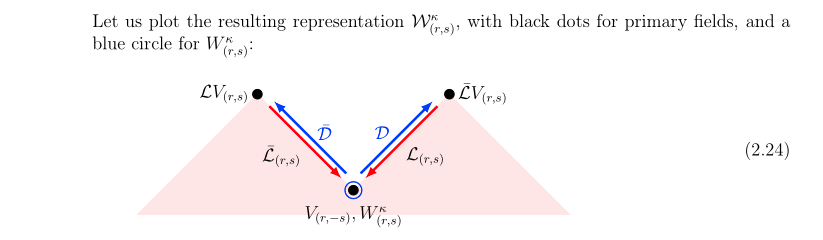
\includegraphics[width=.9\linewidth]{./imgs/logarithmic_module.png}
\end{center}

\(\mathcal L V_{(r,s)}\) and \(\bar{\mathcal L} V_{(r,s)}\) are non-diagonal primary fields. The parameter \(\kappa\) is fixed in the presence of \(V^d_{\langle1,2\rangle}\), in which case the logarithmic module is generated by

\begin{align}
  W^{-}_{(r,s)} = \partial_{P} V_{P_{(r,-s)}} - \mathcal{L}_{(r,s)} \bar{\mathcal{L}}_{(r,s)} \partial_{P} V_{P_{(r,s)}}
\end{align}

This is the necessary condition for the OPE

\begin{align}
  V^{d}_{\langle 1,s_{0}\rangle} V_{P_{(r,0)}+\epsilon}
\end{align}

to be finite.
\subsubsection*{Logarithmic blocks on the sphere}
\label{sec:org48ae354}

The expression of logarithmic four-point blocks on the sphere can be found by assuming the holomorphicity of the 4-point function

\begin{align}
 Z(P) = \sum_{k\in\mathbb{Z}} D_{P+k\beta^{-1}} \left|\mathcal{F}_{P+k\beta^{-1}}\right|^2 +\sum_{r=1}^\infty \sum_{s\in\frac{1}{r}\mathbb{Z}} D_{(r,s)}(P) \mathcal{G}_{(r,s)}\ .
\end{align}

(argument made by Sylvain in the \href{file:///Users/Paul/Documents/Cours suivis/Sylvain CFT review/CFT-Review/solvable.pdf}{solvable.pdf} file on \href{https://github.com/ribault/CFT-Review}{GitHub}).

The coefficient \(D_P\) has a double pole at \(P_{(r,-s)}\). The blocks \(\mathcal F_{P}\) have a simple pole at \(P_{(r,s)}\), and we write

\begin{align}
  \mathcal{F}_{P} = \frac{R_{r,s}}{P-P_{(r,s)}} \mathcal{F}_{P_{(r,-s)}} + \mathcal{F}^{\text{reg}}_{P_{(r,s)}} + O(P-P_{(r,s)}).
\end{align}

Explicitly, using Zamolodchikov's recursion, \(\mathcal F^{\text{reg}}\) is written as

\begin{align}
  \mathcal{F}^{\text{reg}}_{P_{(r,s)}} = (\text{prefactor}) H^{\text{reg}}_{P_{(r,s)}},
\end{align}

where the prefactor is the prefactor in Zamolodchikov's recursion, and

\begin{align}
  H^{\text{reg}}_{P_{(r,s)}} = 1 + \sum_{m,n} \left( \frac{1}{P^{2}_{(r,s)} - P^{2}_{(m,n)}} \right)^{\text{reg}} (16q)^{mn} R_{m,n} H_{P_{(m,-n)}}
\end{align}

and

\begin{align}
\left( \frac{1}{P^{2}_{(r,s)} - P^{2}_{(m,n)}} \right)^{\text{reg}} =
\begin{cases}
\log 16q - \frac{1}{4P_{(r,s)}^{2}} \text{  if  } (m,n)=(r,s) \\
\frac{1}{P^{2}_{(r,s)} - P^{2}_{(m,n)}}  \text{  otherwise}
\end{cases}.
\end{align}


Analysing the poles of this expression (there are double poles and simple ones), one arrives at the following expression for the logarithmic blocks: for \((r, s) \in \mathbb{N}^{*}\),

\begin{align}\label{eq:log_block}
\mathcal{G}_{(r,s)} = (\mathcal{F}_{P_{(r,s)}}^{\text{reg}} - R_{r,s}& \mathcal{F}^{'}_{P_{(r,-s)}}) \bar{\mathcal{F}}_{P_{(r,-s)}} + \frac{R_{r,s}}{\bar R_{r,s}} \mathcal{F}_{P_{(r,-s)}} (\bar{\mathcal{F}}_{P_{(r,s)}}^{\text{reg}} - \bar{R}_{r,s} \bar{\mathcal{F}}^{'}_{P_{(r,-s)}})\nonumber \\
& +R_{r,s} \underbrace{\left( \frac{D^{'}_{P_{(r,s)}}}{D_{P_{(r,s)}}} - \lim_{P \to P_{(r,-s)}} \left[ \frac{2}{P-P_{(r,-s)}} + \frac{D_{P}^{'}}{D_{P}} \right] \right)}_{-\ell^{(1)-}_{(r,s)}}\left|\mathcal{F}_{P_{(r,-s)}}\right|^{2},
\end{align}

in which the primes denote derivatives with respect to the momentum \(P\). The derivative of the block is

\begin{align}
  \mathcal{F}_{P_{(r,-s)}}^{'} = (\text{prefactor}) H^{\text{der}}_{P_{(r,-s)}}, \quad \text{where} \quad H^{\text{der}}_{P} = 2P\log(16q) H_{P} + H_{P}^{'}.
\end{align}

The term \(\ell^{(1)-}_{(r,s)}\) can be computed as the order 1 term in the Taylor expansion of

\begin{align}
  \log \left( \epsilon^{2} \frac{D_{P_{(r,-s)}+\epsilon}}{D_{P_{(r,s)+\epsilon}}} \right) = \sum_{n\geq 0} \ell^{(n)-}_{(r,s)} \epsilon^{n}.
\end{align}

Explicitly,

\begin{align}
 \beta\ell^{(1)-}_{(r,s)} = 4\sum_{j=1-s}^s &\Big\{ \psi(-2\beta^{-1}P_{(r,j)}) +\psi(2\beta^{-1}P_{( r,-j)}) \Big\}
 -4\pi \cot(\pi s \beta^{-2})
 \\
 &-\sum_{j\overset{2}{=}1-s}^{s-1}\sum_{\pm,\pm}\Big\{
 \psi\left(\tfrac12-\beta^{-1}(P_{( r,j)}\pm P_1\pm P_2)\right)
 + \psi\left(\tfrac12+\beta^{-1}(P_{( r,j)}\pm \bar P_1\pm \bar P_2)\right)
 \Big\}
 \\
 &-\sum_{j\overset{2}{=}1-s}^{s-1}\sum_{\pm,\pm}\Big\{
 \psi\left(\tfrac12-\beta^{-1}(P_{( r,j)}\pm P_3\pm P_4)\right)
 + \psi\left(\tfrac12+\beta^{-1}(P_{( r,j)}\pm \bar P_3\pm \bar P_4)\right)
 \Big\}
\end{align}

For \((r, s) \in \mathbb{N}^{*}\), \(\mathcal G_{(r,s)}\) can actually be non-logarithmic, due to residues \(R_{(r,s)}\) and \(\bar R_{(r,s)}\) vanishing.
\subsubsection*{Logarithmic blocks on the torus}
\label{sec:org0ffb68a}

The argument we used for computing logarithmic blocks on the sphere can be transferred verbatim to the case of one point blocks on the torus. In particular, the \ref{eq:log_block} of the logarithmic block is also valid for the torus one-point block, if we replace \(D_P\) by the corresponding structure constant on the torus, namely

\begin{align}
  D_{P} \to \frac{C^{\text{ref}}_{P,P, P_1}}{B_{P}}
\end{align}

where \(P_1\) is the momentum of the external field.
\subsection{Relation between sphere four-point blocks and torus one-point blocks}
\label{sec:orgceef356}
The recursion formulas for torus one-point blocks and sphere four-point blocks imply that four point blocks on the sphere are related to one-point blocks on the torus through the relation

\begin{align}
H^{\text{torus}}_{P}(\tau, c | P_{1} | q^{2}) = H_{\sqrt{2}P}\left(c' \left|\left. P_{(0,\frac12)}, \frac{P_{1}}{\sqrt{2}}, P_{(0,\frac12)}, P_{(0,\frac12)} \right.\right| q \right)
\end{align}

where
\begin{itemize}
\item \(c'\) is related to \(c\) via \(\beta'=\frac\beta{\sqrt 2}\).
\item Fields on the RHS have dimensions \(\Delta = \frac{c'-1}{24} - P^2\).
\end{itemize}

Our code successfully reproduces this relation:

\begin{Code}
\begin{Verbatim}
\color{EFD}\EFk{import} Pkg; Pkg.activate(\EFs{"."})
\EFk{using} JuliVirBootstrap, BenchmarkTools, EllipticFunctions
\EFk{import} JuliVirBootstrap.FourPointBlocksSphere.qfromx
q = JuliVirBootstrap.FourPointBlocksSphere.qfromx(\EFhn{0.05})

left=\EFhn{1};
right=\EFhn{2};
c\_torus = CentralCharge(\EFs{"b"}, \EFhn{1.2}\EFt{+}.\EFhn{1}\EFt{*}\EFhn{1}im);
c\_sphere = CentralCharge(\EFs{"b"}, (\EFhn{1.2}\EFt{+}.\EFhn{1}\EFt{*}\EFhn{1}im)\EFt{/}sqrt(\EFhn{2}))

P = \EFhn{0.23}\EFt{+}.\EFhn{11}im
P1 = \EFhn{0.41}\EFt{+}\EFhn{1.03}im
V\_torus\_chan = Field(c\_torus, \EFs{"P"}, P, diagonal=\EFo{true})
δ\_torus = V\_torus\_chan[\EFs{"δ"}][left]
δ11\_torus = Field(c\_torus, Kac=\EFo{true}, r=\EFhn{1}, s=\EFhn{1}, diagonal=\EFo{true})[\EFs{"δ"}][left]
V\_torus\_ext = Field(c\_torus, \EFs{"P"}, P1, diagonal=\EFo{true})
corr\_torus = OnePointCorrelation

V\_sphere\_chan = Field(c\_sphere, \EFs{"P"}, sqrt(\EFhn{2})\EFt{*}P, diagonal=\EFo{true})
δ\_sphere = V\_sphere\_chan[\EFs{"δ"}][left]
δ21\_sphere = Field(c\_sphere, Kac=\EFo{true}, r=\EFhn{2}, s=\EFhn{1}, diagonal=\EFo{true})[\EFs{"δ"}][left]
δ12\_sphere = Field(c\_sphere, Kac=\EFo{true}, r=\EFhn{1}, s=\EFhn{2}, diagonal=\EFo{true})[\EFs{"δ"}][left]
V\_sphere\_ext = Field(c\_sphere, \EFs{"P"}, P1\EFt{/}sqrt(\EFhn{2}), diagonal=\EFo{true})
VKac\_sphere = Field(c\_sphere, Kac=\EFo{true}, r=\EFhn{0}, s=\EFhn{1}\EFt{//}\EFhn{2}, diagonal=\EFo{true})

corr\_torus = OnePointCorrelation(c\_torus, V\_torus\_ext)
block\_torus = OnePointBlockTorus(V\_torus\_chan)

corr\_sphere = FourPointCorrelation(c\_sphere, [VKac\_sphere, V\_sphere\_ext, VKac\_sphere,VKac\_sphere])
block\_sphere = FourPointBlockSphere(\EFs{"s"}, V\_sphere\_chan)

h1 = JuliVirBootstrap.OnePointBlocksTorus.H(q\EFt{\char94{}}\EFhn{2}, \EFhn{5}, block\_torus, corr\_torus, left)
h2 = JuliVirBootstrap.FourPointBlocksSphere.H(q, \EFhn{5}, block\_sphere, corr\_sphere, left)
\end{Verbatim}
\end{Code}

\begin{Code}
\begin{Verbatim}
\color{EFD}println(\EFs{"torus block = \$h1"})
println(\EFs{"sphere block = \$h2"})
\end{Verbatim}
\end{Code}
torus block = 1.0000059915273005 - 1.1912765043504052e-5im
sphere block = 1.000005991527301 - 1.1912765042311957e-5im
\subsection{Crossing symmetry for four-point functions on the sphere}
\label{sec:org8b7f227}

\subsection{Modular invariance for one-point functions on the torus}
\label{sec:org6624903}
\section{Code of the package\hfill{}\textsc{noeval}}
\label{sec:orgaf4743d}

\subsection{Main module}
\label{sec:orga85c686}
The module \texttt{JuliVirBootstrap} is the main module of this package, and it includes the sub-modules.

\begin{itemize}
\item \texttt{CFTData} provides types for central charges and fields.
\item \texttt{CorrelationFunctions} provides types for one-point and four-point correlation functions, as well as methods for computing coefficients appearing in their conformal blocks.
\item \texttt{VirasoroConformalBlocks} provides types for representing four-point conformal blocks on the sphere and one-point conformal blocks on the torus, as well as methods for computing them.
\end{itemize}

\begin{Code}
\begin{Verbatim}
\color{EFD}\EFcd{\#}\EFc{===========================================================================================}

\EFc{Written by Paul Roux, adapting a Python code written by Sylvain Ribault \& Rongvoram}
\EFc{Nivesvivat}

\EFc{===========================================================================================\#}

\EFk{module} JuliVirBootstrap

\EFcd{\#}\EFc{===========================================================================================}
\EFc{Special functions}
\EFc{===========================================================================================\#}
include(\EFs{"SpecialFunctions.jl"})
\EFk{using} .SpecialFunctions
\EFk{export} Barnes\_G
\EFk{export} log\_double\_Gamma, double\_Gamma

\EFcd{\#}\EFc{===========================================================================================}
\EFc{Central charges and fields}
\EFc{===========================================================================================\#}
include(\EFs{"CFTData.jl"})
\EFk{using} .CFTData
\EFk{export} CentralCharge
\EFk{export} Field, spin

\EFcd{\#}\EFc{===========================================================================================}
\EFc{Correlation functions}
\EFc{===========================================================================================\#}
include(\EFs{"CorrelationFunctions.jl"})
\EFk{using} .FourPointCorrelationFunctions
\EFk{export} FourPointCorrelation

\EFk{using} .OnePointCorrelationFunctions
\EFk{export} OnePointCorrelation

\EFcd{\#}\EFc{===========================================================================================}
\EFc{Conformal blocks}
\EFc{===========================================================================================\#}
include(\EFs{"ConformalBlocks.jl"})
\EFk{using} .FourPointBlocksSphere
\EFk{export} FourPointBlockSphere
\EFk{export} block\_chiral, block\_non\_chiral

\EFk{using} .OnePointBlocksTorus
\EFk{export} OnePointBlockTorus

\EFk{end}
\end{Verbatim}
\end{Code}
\subsection{The \texttt{SpecialFunctions} module}
\label{sec:org114e461}
\subsubsection*{Header}
\label{sec:orgf51f058}

\begin{Code}
\begin{Verbatim}
\color{EFD}\EFcd{\#}\EFc{==================}

\EFc{SpecialFunctions.jl computes the special functions relevant for our applications in 2D CFT.}

\EFc{==================\#}

\EFk{module} SpecialFunctions

\EFk{using} SpecialFunctions \EFcd{\#} \EFc{external Julia package (the module name is the same but there is no domain conflict)}
\EFk{using} Memoization
\EFk{using} ArbNumerics \EFcd{\#} \EFc{the SpecialFunctions package has no arbitrary-precision complex-variable gamma function, however the ArbNumerics does. We use this, and convert to a Complex\{BigFloat\}}
\EFk{using} QuadGK \EFcd{\#} \EFc{numerical integration}

\EFk{export} digamma\_reg, Barnes\_G, log\_double\_Gamma, double\_Gamma

\EFk{function} \EFf{log\_Γ}(z)
    \EFk{return} Complex\{BigFloat\}(lgamma(ArbComplex(z)))
\EFk{end}

\EFk{function} \EFf{Γ}(z)
    \EFk{return} Complex\{BigFloat\}(gamma(ArbComplex(z)))
\EFk{end}

\EFk{function} \EFf{ψ}(z)
    \EFk{return} Complex\{BigFloat\}(digamma(ArbComplex(z)))
\EFk{end}

\EFk{function} \EFf{trigamma}(z)
    \EFk{return} Complex\{BigFloat\}(polygamma(ArbComplex(\EFhn{1}), ArbComplex(z)))
\EFk{end}

\EFk{function} \EFf{polyΓ}(n, z)
    \EFk{return} Complex\{BigFloat\}(polygamma(ArbComplex(n), ArbComplex(z)))
\EFk{end}
\end{Verbatim}
\end{Code}
\subsubsection*{Regularized digamma Function}
\label{sec:org902abd8}

\begin{Code}
\begin{Verbatim}
\color{EFD}\EFs{"""Regularised digamma function"""}
\EFk{function} \EFf{digamma\_reg}(z)
    \EFk{if} real(z) \EFt{>} \EFhn{0}
        \EFk{return} ψ(z)
    \EFk{elseif} imag(z) \EFt{==} \EFhn{0} \EFt{\&\&} real(z)\EFt{\%}\EFhn{1} \EFt{==} \EFhn{0}
        \EFk{return} ψ(\EFhn{1}\EFt{-}z)
    \EFk{else}
        \EFk{return} ψ(\EFhn{1}\EFt{-}z) \EFt{-} big(π)\EFt{/}tan(π\EFt{*}z)
    \EFk{end}
\EFk{end}
\end{Verbatim}
\end{Code}
\subsubsection*{Double gamma function}
\label{sec:org1873129}

The function \texttt{log\_Barnes\_GN} is the logarithm of the function \eqref{eq:Barnes_{GN}}.

\begin{Code}
\begin{Verbatim}
\color{EFD}\EFk{function} \EFf{integrand\_C}(x, τ)
    x = big(x)
    \EFk{return} exp((\EFhn{1}\EFt{-}τ)\EFt{*}x)\EFt{/}(\EFhn{2}\EFt{*}sinh(x)\EFt{*}sinh(τ\EFt{*}x)) \EFt{-} exp(\EFt{-}\EFhn{2}\EFt{*}x)\EFt{/}(τ\EFt{*}x)\EFt{*}(exp(x)\EFt{/}(\EFhn{2}\EFt{*}sinh(x))\EFt{+}\EFhn{1}\EFt{-}τ\EFt{/}\EFhn{2})
\EFk{end}

\EFk{function} \EFf{modular\_C}(τ)
    P = precision(BigFloat, base=\EFhn{10})
    \EFcd{\#}\EFc{temporarily increase precision to avoid artificial divergence around zero}
    setprecision(BigFloat, base=\EFhn{10}, Int(floor(\EFhn{1.3}\EFt{*}P)))
    cutoff = big(\EFhn{10}\EFt{\char94{}}(\EFt{-}P\EFt{/}\EFhn{5})) \EFcd{\#} \EFc{to prevent artificial divergence around zero}
    tol = big(\EFhn{10})\EFt{\char94{}}P
    value, error = quadgk(x \EFt{->} integrand\_C(x, τ), cutoff, big(\EFo{Inf}), rtol = tol, order=\EFhn{21})
    C0 = (\EFhn{2}\EFt{/}τ \EFt{-} \EFhn{3}\EFt{//}\EFhn{2} \EFt{+} τ\EFt{/}\EFhn{6})\EFt{*}cutoff \EFt{+} (\EFhn{5}\EFt{//}\EFhn{12} \EFt{-} \EFhn{1}\EFt{/}τ \EFt{+} τ\EFt{/}\EFhn{12})\EFt{*}cutoff\EFt{\char94{}}\EFhn{2} \EFt{+} (\EFhn{4}\EFt{/}(\EFhn{9}\EFt{*}τ) \EFt{-} \EFhn{2}\EFt{//}\EFhn{9} \EFt{+} \EFhn{1}\EFt{//}\EFhn{54}\EFt{*}τ \EFt{-} \EFhn{1}\EFt{//}\EFhn{270}\EFt{*}τ\EFt{\char94{}}\EFhn{3})\EFt{*}cutoff\EFt{\char94{}}\EFhn{3}
    setprecision(BigFloat, base=\EFhn{10}, P)
    \EFk{return} \EFhn{1}\EFt{/}(\EFhn{2}\EFt{*}τ)\EFt{*}log(\EFhn{2}\EFt{*}big(π)) \EFt{-} value \EFt{-} C0
\EFk{end}

\EFk{function} \EFf{integrand\_D}(x, τ)
    x = big(x)
    \EFk{return} x\EFt{*}exp((\EFhn{1}\EFt{-}τ)\EFt{*}x)\EFt{/}(sinh(x)\EFt{*}sinh(τ\EFt{*}x)) \EFt{-} exp(\EFt{-}\EFhn{2}\EFt{*}x)\EFt{/}(τ\EFt{*}x)
\EFk{end}

\EFk{function} \EFf{modular\_D}(τ)
    P = precision(BigFloat, base=\EFhn{10})
    \EFcd{\#}\EFc{temporarily increase precision to avoid artificial divergence around zero}
    setprecision(BigFloat, base=\EFhn{10}, Int(floor(\EFhn{1.3}\EFt{*}P)))
    cutoff = big(\EFhn{10}\EFt{\char94{}}(\EFt{-}P\EFt{/}\EFhn{5})) \EFcd{\#} \EFc{to prevent artificial divergence around zero}
    tol = big(\EFhn{10})\EFt{\char94{}}P
    value, error = quadgk( x \EFt{->} integrand\_D(x, τ), big(\EFhn{0}), big(\EFo{Inf}), rtol = tol, order=\EFhn{21})
    setprecision(BigFloat, base=\EFhn{10}, P)
    \EFk{return} value
\EFk{end}

\textcolor[HTML]{483d8b}{\textbf{@memoize}} \EFk{function} modular\_coeff\_a(τ)
    \EFk{return} \EFhn{1}\EFt{/}\EFhn{2}\EFt{*}τ\EFt{*}log(big(\EFhn{2})\EFt{*}π\EFt{*}τ) \EFt{+} \EFhn{1}\EFt{/}\EFhn{2}\EFt{*}log(τ) \EFt{-} τ\EFt{*}modular\_C(τ)
\EFk{end}

\textcolor[HTML]{483d8b}{\textbf{@memoize}} \EFk{function} modular\_coeff\_b(τ)
    \EFk{return} \EFt{-}τ\EFt{*}log(τ) \EFt{-} τ\EFt{\char94{}}\EFhn{2}\EFt{*}modular\_D(τ)
\EFk{end}

\EFk{function} \EFf{log\_Barnes\_GN}(N, z, τ)
    res = \EFhn{0}
    res \EFt{+=} \EFt{-} log(τ) \EFt{-} log\_Γ(z)
    res \EFt{+=} modular\_coeff\_a(τ)\EFt{*}z\EFt{/}τ \EFt{+} modular\_coeff\_b(τ)\EFt{*}z\EFt{\char94{}}\EFhn{2}\EFt{/}(\EFhn{2}\EFt{*}τ\EFt{\char94{}}\EFhn{2})
    res \EFt{+=} sum(log\_Γ(m\EFt{*}τ) \EFt{-} log\_Γ(z\EFt{+}m\EFt{*}τ) \EFt{+} z\EFt{*}ψ(m\EFt{*}τ)\EFt{+}z\EFt{\char94{}}\EFhn{2}\EFt{/}\EFhn{2}\EFt{*}trigamma(m\EFt{*}τ) \EFk{for} m \EFk{in} \EFhn{1}:N)
    \EFk{return} res
\EFk{end}

\textcolor[HTML]{483d8b}{\textbf{@memoize}} \EFk{function} factorial\_big(n)\EFt{::BigInt}
    \EFk{return} factorial(big(n))
\EFk{end}

\textcolor[HTML]{483d8b}{\textbf{@memoize}} \EFk{function} polynomial\_Pn(n, z, τ)
    \EFk{if} n \EFt{==} \EFhn{1}
        \EFk{return} \EFhn{1}\EFt{//}\EFhn{6}
    \EFk{else}
        term1 = z\EFt{\char94{}}(n\EFt{-}\EFhn{1})\EFt{/}factorial\_big(n\EFt{+}\EFhn{2})
        \EFf{summand}(k) = ((\EFhn{1}\EFt{+}τ)\EFt{\char94{}}(k\EFt{+}\EFhn{2}) \EFt{-} \EFhn{1} \EFt{-} τ\EFt{\char94{}}(k\EFt{+}\EFhn{2}))\EFt{/}(factorial\_big(k\EFt{+}\EFhn{2})\EFt{*}τ) \EFt{*} polynomial\_Pn(n\EFt{-}k, z, τ)
        \EFk{return} term1 \EFt{-} sum(summand(k) \EFk{for} k \EFk{in} \EFhn{1}:n\EFt{-}\EFhn{1})
    \EFk{end}
\EFk{end}

\EFk{function} \EFf{rest\_RMN}(M, N, z, τ)
    \EFk{return} sum(factorial\_big(k\EFt{-}\EFhn{1})\EFt{*}(\EFt{-}τ)\EFt{\char94{}}(\EFt{-}k\EFt{-}\EFhn{1})\EFt{*}polynomial\_Pn(k, z, \EFt{-}τ)\EFt{/}N\EFt{\char94{}}k \EFk{for} k \EFk{in} \EFhn{1}:M)
\EFk{end}

\EFs{"""Numerical approximation of the logarithm of Barne's G-function, up to a given tolerance"""}
\EFk{function} \EFf{log\_Barnes\_G}(z, τ, tol)
    z = complex(z)
    d = \EFt{-}log(tol)\EFt{/}log(\EFhn{10})
    M = BigInt(floor(\EFhn{0.7}\EFt{*}log(\EFhn{10})\EFt{/}log(\EFhn{20})\EFt{*}d))
    N = \EFhn{20}\EFt{*}M
    \EFk{return} log\_Barnes\_GN(N, z, τ) \EFt{+} z\EFt{\char94{}}\EFhn{3}\EFt{*}rest\_RMN(M, N, z, τ)
\EFk{end}

\EFk{function} \EFf{Barnes\_G}(z, τ, tol)
    \EFk{return} exp(log\_Barnes\_G(z, τ, tol))
\EFk{end}

\EFk{function} \EFf{log\_Gamma\_2}(w, β, tol)
    β = real(β\EFt{-}\EFhn{1}\EFt{/}β) \EFt{<} \EFhn{0} \EFk{?} \EFhn{1}\EFt{/}β \EFk{:} β \EFcd{\#} \EFc{change β -> 1/β if needed}
    \EFk{return} w\EFt{/}(\EFhn{2}\EFt{*}β)\EFt{*}log(big(\EFhn{2})\EFt{*}π) \EFt{+} (w\EFt{/}\EFhn{2}\EFt{*}(w\EFt{-}β\EFt{-}\EFhn{1}\EFt{/}β)\EFt{+}\EFhn{1})\EFt{*}log(β) \EFt{-} log\_Barnes\_G(w\EFt{/}β, \EFhn{1}\EFt{/}β\EFt{\char94{}}\EFhn{2}, tol)
\EFk{end}

\EFs{"""}
        \EFs{log\_double\_Gamma(w, β, tol)}

\EFs{Compute the logarithm of the double gamma function Γ\_β(w, β) with precision tol}

\EFs{"""}
\EFk{function} \EFf{log\_double\_Gamma}(w, β, tol)
    \EFk{return} log\_Gamma\_2(w, β, tol) \EFt{-} log\_Gamma\_2((β\EFt{+}\EFhn{1}\EFt{/}β)\EFt{/}\EFhn{2}, β, tol)
\EFk{end}

\EFs{"""}
        \EFs{double\_Gamma(w, β, tol)}

\EFs{Compute the double gamma function Γ\_β(w, β) with precision tol}

\EFs{"""}
\EFk{function} \EFf{double\_Gamma}(w, β, tol)
    exp(log\_double\_Gamma(w, β, tol))
\EFk{end}
\end{Verbatim}
\end{Code}
\subsubsection*{End module}
\label{sec:org4a773f4}

\begin{Code}
\begin{Verbatim}
\color{EFD}\EFk{end} \EFcd{\#} \EFc{end module}
\end{Verbatim}
\end{Code}
\subsection{The \texttt{CFTData} module}
\label{sec:orge424e13}
The file \href{src/CFTData.jl}{CFTData.jl} defines
\begin{itemize}
\item a struct \texttt{CentralCharge} that represents a central charge \(c\) and contains the value of the four corresponding parameters \(b, B, \beta, c\)
\item a struct \texttt{Field} that represents a field \(V\). The field can be defined from its Kac indices \(r, s\), be diagonal, logarithmic, or degenerate. The struct contains booleans for these three characteristics, as well as rationals for \(r\) and \(s\), and the pairs of (left, right) values \((\Delta, \bar \Delta)\), \((p, \bar p)\), \((\delta, \bar \delta)\), \((P, \bar P)\).
\end{itemize}
\subsubsection*{Header}
\label{sec:org6e4771e}

\begin{Code}
\begin{Verbatim}
\color{EFD}
\EFcd{\#}\EFc{===========================================================================================}

\EFc{CFTData.jl contains a module CFTData that provides types representing}
\EFc{central charges and fields in 2D CFTs with Virasoro symmetry.}

\EFc{Written by Paul Roux, adapting a Python code written by Sylvain Ribault \& Rongvoram}
\EFc{Nivesvivat}

\EFc{============================================================================================\#}

\EFs{"""}
\EFs{Provides types representing central charges and fields in CFT.}
\EFs{"""}
\EFk{module} CFTData

\EFk{using} Match;

\EFk{export} CentralCharge, Field, spin

\EFs{"""print complex numbers in latex format"""}
\EFk{function} Base.\EFf{show}(io\EFt{::IO},\EFt{::MIME}\EFs{"text/latex"},z\EFt{::Complex})
    print(\EFs{"\$(real(z)) + \$(imag(z))i"})
\EFk{end}

\end{Verbatim}
\end{Code}
\subsubsection*{Central charge}
\label{sec:org23e754e}

\begin{Code}
\begin{Verbatim}
\color{EFD}\EFs{"""Get B from given parameter"""}
\EFk{function} \EFf{Bfrom}(parameter, value)
    \textcolor[HTML]{483d8b}{\textbf{@match}} parameter \EFk{begin}
        \EFs{"c"} \EFt{=>} (value\EFt{-}\EFhn{13}\EFt{+}sqrt(complex((value\EFt{-}\EFhn{1})\EFt{*}(value\EFt{-}\EFhn{25}))))\EFt{/}\EFhn{12}
        \EFs{"b"} \EFt{=>} value\EFt{\char94{}}\EFhn{2}
        \EFs{"β"} \EFt{=>} \EFt{-}value\EFt{\char94{}}\EFhn{2}
        \EFs{"B"} \EFt{=>} value
    \EFk{end}
\EFk{end}

\EFs{"""Get asked parameter from B"""}
\EFk{function} \EFf{Bto}(parameter, value)
    \textcolor[HTML]{483d8b}{\textbf{@match}} parameter \EFk{begin}
        \EFs{"c"} \EFt{=>} \EFhn{13}\EFt{+}\EFhn{6}\EFt{*}value\EFt{+}\EFhn{6}\EFt{/}value
        \EFs{"b"} \EFt{=>} \EFt{-}sqrt(complex(value))
        \EFs{"β"} \EFt{=>} \EFt{-}im\EFt{*}sqrt(complex(value))
        \EFs{"B"} \EFt{=>} value
    \EFk{end}
\EFk{end}

\EFs{"""}
    \EFs{CentralCharge\{T\}}
\EFs{Object representing the central charge.}
\EFs{Contains the values of the 4 parameters representing it.}
\EFs{"""}
\EFk{struct} \EFt{CentralCharge}\{T\}

    \EFcd{\#}\EFc{= T is the type of the parameters; either Complex\{Float64\} or Complex\{BigFloat\}}
    \EFc{for arbitrary precision. =\#}
    values\EFt{::Dict}\{String, T\}

\EFk{end}

\EFs{"""}
    \EFs{CentralCharge(parameter, value)}

\EFs{Constructor function for the CentralCharge type.}

\EFs{Given one of the four parameters `"c"`, `"b"`, `"β"`, `"B"` and its value,}
\EFs{creates an object CentralCharge\{T\} where T is the type of `value`.}

\EFs{\# Example}
\EFs{```julia-repl}
\EFs{julia> setprecision(BigFloat, 20, base=10)}
\EFs{julia> charge = CentralCharge("β", sqrt(big(2)))}
\EFs{Central charge :}
\EFs{B = -2.0 + 0.0im}
\EFs{c = -2.0 + 0.0im}
\EFs{b = 0.0 + 1.414213562373095048804im}
\EFs{β = -1.414213562373095048804 + 0.0im}
\EFs{```}
\EFs{"""}
\EFk{function} \EFf{CentralCharge}(parameter = \EFs{"c"}, value = \EFhn{1})
    \EFcd{\#} \EFc{Constructor}
    T=typeof(AbstractFloat(real(value)))
    B=Bfrom(parameter, value)
    dict=Dict(key \EFt{=>} Bto(key, B) \EFk{for} key \EFk{in} (\EFs{"c"}, \EFs{"b"}, \EFs{"β"}, \EFs{"B"}))
    CentralCharge\{complex(T)\}(dict)
\EFk{end}
\end{Verbatim}
\end{Code}
\begin{itemize}
\item Pretty printing
\label{sec:orgf93c64e}

\begin{Code}
\begin{Verbatim}
\color{EFD}\EFs{"""Display an object of type CentralCharge"""}
\EFk{function} Base.\EFf{show}(io\EFt{::IO}, charge\EFt{::CentralCharge})
    println(\EFs{"Central charge:"})
    \EFk{for} (key, value) \EFk{in} charge.values
        println(io, \EFs{"\$key = \$value"})
    \EFk{end}
\EFk{end}

\EFs{"""Display the value of the central charge in LaTeX format"""}
\EFk{function} Base.\EFf{show}(io\EFt{::IO}, \EFt{::MIME}\EFs{"text/latex"}, charge\EFt{::CentralCharge}, parameter)
    \EFk{if} parameter\EFt{==}\EFs{"β"}
        print(\EFs{"\char92{}\char92{}beta = "})
    \EFk{else}
        print(parameter,\EFs{" = "})
    \EFk{end}
    show(io, MIME(\EFs{"text/latex"}), charge[parameter])
\EFk{end}

\EFs{"""Overload of [] to access values in charge"""}
Base.\EFf{getindex}(charge\EFt{::CentralCharge}, key) = charge.values[key];
\end{Verbatim}
\end{Code}
\end{itemize}
\subsubsection*{Fields}
\label{sec:org744e8a7}

Fields can be given from any of the four parameters \(\Delta, \delta, P, p\). Optional keyword arguments lets us choose whether the field is diagonal, degenerate, logarithmic. The field can also be defined from its r and s indices using the keyword argument Kac = true.

\begin{Code}
\begin{Verbatim}
\color{EFD}\EFs{"""Get P from any given parameter"""}
\EFk{function} \EFf{P\_from}(parameter, value, c\EFt{::CentralCharge})
    \textcolor[HTML]{483d8b}{\textbf{@match}} parameter \EFk{begin}
        \EFs{"Δ"} \EFt{=>} sqrt(complex(value \EFt{-} (c[\EFs{"c"}]\EFt{-}\EFhn{1})\EFt{/}\EFhn{24}))
        \EFs{"δ"} \EFt{=>} sqrt(complex(value))
        \EFs{"P"} \EFt{=>} value
        \EFs{"p"} \EFt{=>} im\EFt{*}value
    \EFk{end}
\EFk{end}

\EFs{"""Get all parameters from P"""}
\EFk{function} \EFf{P\_to}(parameter, value, c\EFt{::CentralCharge})
    \textcolor[HTML]{483d8b}{\textbf{@match}} parameter \EFk{begin}
        \EFs{"Δ"} \EFt{=>} value\EFt{\char94{}}\EFhn{2} \EFt{+} (c[\EFs{"c"}]\EFt{-}\EFhn{1})\EFt{/}\EFhn{24}
        \EFs{"δ"} \EFt{=>} value\EFt{\char94{}}\EFhn{2}
        \EFs{"P"} \EFt{=>} value
        \EFs{"p"} \EFt{=>} \EFt{-}im\EFt{*}value
    \EFk{end}
\EFk{end}

\EFs{"""}
    \EFs{Field\{T\}}
\EFs{Object representing a conformal field.}
\EFs{Contains the values of the 4 parameters `"Δ"`,`"δ"`,`"P"`,`"p"` for its conformal dimension,}
\EFs{and flags saying whether the field has declared and rational Kac indices, is degenerate, or diagonal.}
\EFs{"""}
\EFk{struct} \EFt{Field}\{T\}

    values\EFt{::Dict}\{String, Vector\{T\}\}
    isKac\EFt{::Bool}
    r\EFt{::Rational}
    s\EFt{::Rational}
    isdegenerate\EFt{::Bool}
    isdiagonal\EFt{::Bool}

\EFk{end}

\EFs{"""}
   \textcolor[HTML]{ff8e00}{\textbf{TODO:}} \EFs{update the examples}
    \EFs{Field(charge, parameter, leftvalue, rightvalue; kwargs...)}

\EFs{Constructor function for the Field type.}

\EFs{Given a charge `charge`, one of the four parameters `"Δ"`, `"δ"`, `"P"`, `"p"` and two values,}
\EFs{create an object Field\{T\} (where T is the type of the values in `charge`) that represents a}
\EFs{field of left and right dimensions given by leftvalue and rightvalue in the chosen}
\EFs{parametrisation.}
\EFs{If given only one value for the parameters Δ, δ, P or p, the field is diagonal by default}

\EFs{\# keyword arguments:}

\EFs{- `Kac::Bool`: if set to true, the field can be constructed from the values of its r and s}
\EFs{indices. By convention V\_(r,s) has left and right momenta (P\_(r,s), P\_(r,-s))}
\EFs{- `r::Rational`,`s::Rational`: used in conjunction to `Kac=true`, must be given rational}
\EFs{values,}
\EFs{- `degenerate::Bool`: set to True if the field is degenerate,}
\EFs{- `diagonal::Bool`: set to True to get a diagonal field ; only the leftvalue needs to be}
\EFs{given.}

\EFs{\# Examples}
\EFs{```julia-repl}
\EFs{julia> charge = CentralCharge("b", big(0.5));}
\EFs{julia> field = Field(charge, Kac=true, r=0, s=1)}
\EFs{Non-diagonal field with Kac indices r = 0//1, s = 1//1 and (left,right) dimensions:}
\EFs{Δ = ( 2.5625 + 0.0im, 2.5625 + 0.0im )}
\EFs{P = ( -0.0 - 1.0im, 0.0 + 1.0im )}
\EFs{δ = ( 1.0 - 0.0im, 1.0 + 0.0im )}
\EFs{p = ( -1.0 + 0.0im, 1.0 + 0.0im )}
\EFs{```}
\EFs{```julia-repl}
\EFs{julia> charge = CentralCharge("β", 1.5+im);}
\EFs{julia> Field(charge, "δ", 2, 3)}
\EFs{Non-diagonal field with (left, right) dimensions:}
\EFs{Δ = ( 2.1579142011834325 - 0.6789940828402367im, 3.1579142011834316 - 0.6789940828402367im )}
\EFs{P = ( 0.0 + 1.4142135623730951im, 0.0 + 1.7320508075688772im )}
\EFs{δ = ( 2.0000000000000004 + 0.0im, 2.9999999999999996 + 0.0im )}
\EFs{p = ( 1.4142135623730951 + 0.0im, 1.7320508075688772 + 0.0im )}
\EFs{```}
\EFs{```julia-repl}
\EFs{julia> charge = CentralCharge();}
\EFs{julia> Field(charge, "δ", 1, diagonal=true)}
\EFs{Diagonal field of dimension:}
\EFs{Δ = 1.0 + 0.0im}
\EFs{P = 0.0 + 1.0im}
\EFs{δ = 1.0 + 0.0im}
\EFs{p = 1.0 + 0.0im}
\EFs{```}
\EFs{"""}
\EFk{function} \EFf{Field}(
    charge\EFt{::CentralCharge} = CentralCharge(\EFs{"c"}, \EFhn{1}),
    parameter = \EFs{"Δ"},
    leftvalue = \EFhn{0};
    rightvalue = \EFhn{0},
    Kac = \EFo{false}, r = \EFhn{0}, s = \EFhn{0},
    degenerate = \EFo{false},
    diagonal = \EFo{false}
    )

    T=typeof(charge.values[\EFs{"c"}]) \EFcd{\#} \EFc{values of dimensions have the same precision as central charges}
    \EFk{if} \EFt{!}Kac
        diagonal = \EFo{true} \EFcd{\#} \EFc{by default a field not given from Kac indices is diagonal}
    \EFk{end}
    \EFk{if} degenerate \EFcd{\#} \EFc{degenerate fields are diagonal and must be given from Kac indices}
        Kac = \EFo{true}
        diagonal = \EFo{true}
    \EFk{end}
    \EFk{if} Kac
        Pleft = \EFhn{1}\EFt{/}\EFhn{2}\EFt{*}(charge[\EFs{"β"}]\EFt{*}r \EFt{-} \EFhn{1}\EFt{/}charge[\EFs{"β"}]\EFt{*}s)
        Pright = \EFhn{1}\EFt{/}\EFhn{2}\EFt{*}(charge[\EFs{"β"}]\EFt{*}r \EFt{+} \EFhn{1}\EFt{/}charge[\EFs{"β"}]\EFt{*}s)
    \EFk{else}
        Pleft, Pright = P\_from.(parameter, [leftvalue, rightvalue], Ref(charge))
    \EFk{end}
    \EFk{if} diagonal
        Pright = Pleft
    \EFk{end}
    values = Dict(key \EFt{=>} P\_to.(key, [Pleft, Pright], Ref(charge))
                  \EFk{for} key \EFk{in} (\EFs{"Δ"}, \EFs{"δ"}, \EFs{"P"}, \EFs{"p"}))

    Field\{complex(T)\}(values, Kac, r, s, degenerate, diagonal)
\EFk{end}

\EFcd{\#} \EFc{Overload the == operator}
\EFk{function} \EFf{Base}.:(\EFt{==})(V1\EFt{::Field}, V2\EFt{::Field})
    \EFk{return} V1[\EFs{"Δ"}] \EFt{==} V2[\EFs{"Δ"}]
\EFk{end}

\EFs{"""Compute the spin Δleft - Δright of a field."""}
\EFk{function} \EFf{spin}(field\EFt{::Field})\EFt{::Rational}
    \EFk{if} field.isdiagonal
        \EFk{return} \EFhn{0}
    \EFk{elseif} field.isKac
        \EFk{return} field.r\EFt{*}field.s
    \EFk{else} \EFcd{\#} \EFc{this should never happen}
        \EFk{return} field[\EFs{"Δ"}][\EFhn{1}] \EFt{-} field[\EFs{"Δ"}][\EFhn{2}]
    \EFk{end}
\EFk{end}
\end{Verbatim}
\end{Code}
\begin{itemize}
\item Pretty printing
\label{sec:org6d4dba2}

\begin{Code}
\begin{Verbatim}
\color{EFD}\EFs{"""Display field"""}
\EFk{function} Base.\EFf{show}(io\EFt{::IO},field\EFt{::Field})
    \EFcd{\#}\EFc{Print fields}
    \EFk{if} field.isdiagonal
        println(\EFs{"Diagonal field of dimension:"})
        \EFk{for} (key, value) \EFk{in} field.values
            println(io, \EFs{"  \$key = \$(value[1])"})
        \EFk{end}
    \EFk{else}
        print(\EFs{"Non-diagonal field "})
        \EFk{if} field.isKac
            print(\EFs{"with Kac indices\char92{}n  r = \$(field.r)\char92{}n  s = \$(field.s)\char92{}nand "})
        \EFk{else}
            print(\EFs{"with "})
        \EFk{end}
        println(\EFs{"(left, right) dimensions:"})

        println(io, \EFs{"  Δ = (\$(field["}Δ\EFs{"][1]), \$(field["}Δ\EFs{"][2]))"})
    \EFk{end}
\EFk{end}

\EFs{"""Display dimension of field in latex format"""}
\EFk{function} Base.\EFf{show}(io\EFt{::IO},\EFt{::MIME}\EFs{"text/latex"}, field\EFt{::Field},parameter)
    \EFk{if} field.isdiagonal
        \EFk{if} parameter \EFt{==} \EFs{"Δ"}
            print(\EFs{"\char92{}\char92{}Delta = "})
        \EFk{elseif} parameter \EFt{==} \EFs{"δ"}
            print(\EFs{"\char92{}\char92{}delta = "})
        \EFk{else}
            print(parameter,\EFs{" = "})
        \EFk{end}
        show(io, MIME(\EFs{"text/latex"}), field[parameter][\EFhn{1}])
    \EFk{else}
        \EFk{if} parameter\EFt{==}\EFs{"Δ"}
            print(\EFs{"(\char92{}\char92{}Delta, \char92{}\char92{}bar\char92{}\char92{}Delta) = "})
        \EFk{elseif} parameter\EFt{==}\EFs{"δ"}
            print(\EFs{"(\char92{}\char92{}delta, \char92{}\char92{}bar\char92{}\char92{}delta) = "})
        \EFk{else}
            print(\EFs{"(\$parameter, \char92{}\char92{}bar\$parameter) = "})
        \EFk{end}
        print(\EFs{"("}); show(io, MIME(\EFs{"text/latex"}), field[parameter][\EFhn{1}]); print(\EFs{", "});
        show(io, MIME(\EFs{"text/latex"}), field[parameter][\EFhn{2}]); print(\EFs{")"})
    \EFk{end}
\EFk{end}

\EFcd{\#} \EFc{function Base.show(io::IO, arr::Vector\{Field\{T\}\}) where \{T\}}
\EFcd{\#}     \EFc{println(io, "Vector\{Field\{\$T\}\} with \$(length(arr)) elements:")}
\EFcd{\#}     \EFc{for (index, field) in enumerate(arr)}
\EFcd{\#}         \EFc{print(io, "\$(index): ")}
\EFcd{\#}         \EFc{show(io, field)}
\EFcd{\#}         \EFc{println()}
\EFcd{\#}     \EFc{end}
\EFcd{\#} \EFc{end}

\EFs{"""Overload []"""}
Base.\EFf{getindex}(field\EFt{::Field},key) = field.values[key];
\end{Verbatim}
\end{Code}
\end{itemize}
\subsubsection*{End of module}
\label{sec:org0735638}

\begin{Code}
\begin{Verbatim}
\color{EFD}\EFk{end} \EFcd{\#} \EFc{end module}
\end{Verbatim}
\end{Code}
\subsection{The \texttt{FourPointCorrelationFunctions} module}
\label{sec:org2d1cc33}
The module \texttt{FourPointCorrelationFunctions} defines

\begin{itemize}
\item a struct \texttt{FourPointCorrelation} that represents a four point function

\[
  < V_1(0) V_2(1) V_3(\infty) V_4(x)>
  \]

\item a method \texttt{computeCNmn} that computes the coefficients \(C^N_{m,n}\) which serve to compute the conformal blocks that enter the expansion of the 4-pt function.
\end{itemize}
\begin{itemize}
\item Header
\label{sec:org1fb80ab}

\begin{Code}
\begin{Verbatim}
\color{EFD}\EFcd{\#}\EFc{===========================================================================================}

\EFc{Written by Paul Roux, adapting a Python code written by Sylvain Ribault \& Rongvoram}
\EFc{Nivesvivat}

\EFc{===========================================================================================\#}

\EFk{module} FourPointCorrelationFunctions

\EFk{export} FourPointCorrelation, computeCNmn

\EFk{using} ..CFTData
\EFk{using} Match
\EFk{import} Memoization: \textcolor[HTML]{483d8b}{\textbf{@memoize}}
\end{Verbatim}
\end{Code}
\item Four-point correlation type
\label{sec:orgfe72d7b}

We create a struct \texttt{FourPointCorrelation} for representing a four-point function on the sphere, that is, a central charge and four external fields.

\begin{Code}
\begin{Verbatim}
\color{EFD}\EFs{"""Struct representing a four-point function. Contains}
\EFs{- a central charge}
\EFs{- 4 external fields}
\EFs{"""}
\EFk{struct} \EFt{FourPointCorrelation}\{T\}
    charge\EFt{::CentralCharge}\{T\}
    fields\EFt{::Vector}\{Field\{T\}\}
\EFk{end}

\EFk{function} \EFf{FourPointCorrelation}(charge\EFt{::CentralCharge}\{T\}, V1, V2, V3, V4) \EFk{where} \{T\}
    \EFk{return} FourPointCorrelation\{T\}(charge, [V1, V2, V3, V4])
\EFk{end}

\EFs{"""Display a four-point function"""}
\EFk{function} Base.\EFf{show}(io\EFt{::IO}, corr\EFt{::FourPointCorrelation})
    println(\EFs{"Four-point correlation function: < V\_1 V\_2 V\_3 V\_4 > where "})
    print(\EFs{"V\_1 = "}); show(corr.fields[\EFhn{1}])
    print(\EFs{"V\_2 = "}); show(corr.fields[\EFhn{2}])
    print(\EFs{"V\_3 = "}); show(corr.fields[\EFhn{3}])
    print(\EFs{"V\_4 = "}); show(corr.fields[\EFhn{4}])
\EFk{end}

\EFcd{\#} \EFc{explicit names for the indices of left and right dimensions}
\EFk{const} \EFv{left} = \EFhn{1}
\EFk{const} \EFv{right} = \EFhn{2}
\end{Verbatim}
\end{Code}
\item Compute \(C^N_{m,n}\)
\label{sec:org243d2aa}

The function \texttt{permute\_ext\_fields} permutes the external fields such that the first two and last two are fused together in the channel.

The function \texttt{Rmn\_zero\_order} computes the order of a zero of R, to avoid computing 0/0 in \(\frac{R_{m,n}}{\delta - \delta_{r,s}}\). At generic central charge (non-rational) \(R_{m,n}\) is zero iff one of the two pairs of fused fields have Kac indices such that \(r_1 \pm r_2 \in \{1-m, 3-m, \dots, m-1\}\) or \(s_1 \pm s_2 \in \{1-n, 3-n, \dots, n-1\}\).

When \(R_{m,n}=0\), we compute a regularisation of it, i.e. the \(O(\epsilon)\) term in the residue of the conformal block where the channel field's dimension is shifted by \(\epsilon\).

This is given by (some expression)

\begin{align}
&\left(\delta_2-\delta_1\right)_\text{reg} = 2p_2 \\
&\left((\delta_2-\delta_1)^2 -2\delta_{(r,s)}(\delta_1+\delta_2) + \delta_{(r,s)}^2\right)_\text{reg} = 8p_1p_2p_{(r,s)}
\end{align}

\begin{Code}
\begin{Verbatim}
\color{EFD}\EFf{double\_prod\_in\_Dmn}(m, n, B) = prod(prod((r\EFt{\char94{}}\EFhn{2}\EFt{*}B \EFt{-} s\EFt{\char94{}}\EFhn{2}\EFt{/}B)\EFt{\char94{}}\EFhn{2} \EFk{for} s in \EFhn{1}:n\EFt{-}\EFhn{1}) \EFk{for} r \EFk{in} \EFhn{1}:m\EFt{-}\EFhn{1})

\EFf{δrs}(r, s, B) = \EFt{-}\EFhn{1}\EFt{/}\EFhn{4} \EFt{*} (B\EFt{*}r\EFt{\char94{}}\EFhn{2} \EFt{+} \EFhn{2}\EFt{*}r\EFt{*}s \EFt{+} s\EFt{\char94{}}\EFhn{2}\EFt{/}B)

\EFk{function} \EFf{Dmn}(m, n, B)
    \EFk{if} m \EFt{==} \EFhn{1} \EFt{\&\&} n \EFt{==} \EFhn{1} \EFcd{\#} \EFc{treat cases m = 1, n=1 separately}
        \EFk{return} \EFhn{1}
    \EFk{elseif} m \EFt{==} \EFhn{1}
        \EFk{return} n \EFt{*} prod(s\EFt{\char94{}}\EFhn{2}\EFt{/}B \EFt{*} (s\EFt{\char94{}}\EFhn{2}\EFt{/}B \EFt{-} m\EFt{\char94{}}\EFhn{2}\EFt{*}B) \EFk{for} s \EFk{in} \EFhn{1}:n\EFt{-}\EFhn{1})
    \EFk{elseif} n \EFt{==} \EFhn{1}
        \EFk{return} m \EFt{*} prod(r\EFt{\char94{}}\EFhn{2}\EFt{*}B \EFt{*} (r\EFt{\char94{}}\EFhn{2}\EFt{*}B \EFt{-} n\EFt{\char94{}}\EFhn{2}\EFt{/}B) \EFk{for} r \EFk{in} \EFhn{1}:m\EFt{-}\EFhn{1})
    \EFk{else}
        f1 = prod(r\EFt{\char94{}}\EFhn{2}\EFt{*}B \EFt{*} (r\EFt{\char94{}}\EFhn{2}\EFt{*}B \EFt{-} n\EFt{\char94{}}\EFhn{2}\EFt{/}B) \EFk{for} r \EFk{in} \EFhn{1}:m\EFt{-}\EFhn{1})
        f2 = prod(s\EFt{\char94{}}\EFhn{2}\EFt{/}B \EFt{*} (s\EFt{\char94{}}\EFhn{2}\EFt{/}B \EFt{-} m\EFt{\char94{}}\EFhn{2}\EFt{*}B) \EFk{for} s \EFk{in} \EFhn{1}:n\EFt{-}\EFhn{1})
        f3 = double\_prod\_in\_Dmn(m, n, B)
        \EFk{return} m\EFt{*}n\EFt{*}f1\EFt{*}f2\EFt{*}f3
    \EFk{end}
\EFk{end}

\EFs{"""Permute the external fields to get t- or u-channels from s-channel"""}
\EFk{function} \EFf{permute\_ext\_fields}(corr\EFt{::FourPointCorrelation}, channel)
    Vs=corr.fields
    Vs = \textcolor[HTML]{483d8b}{\textbf{@match}} channel \EFk{begin}
        \EFs{"s"} \EFt{=>} [Vs[\EFhn{1}], Vs[\EFhn{2}], Vs[\EFhn{3}], Vs[\EFhn{4}]]
        \EFs{"t"} \EFt{=>} [Vs[\EFhn{1}], Vs[\EFhn{4}], Vs[\EFhn{3}], Vs[\EFhn{2}]]
        \EFs{"u"} \EFt{=>} [Vs[\EFhn{1}], Vs[\EFhn{3}], Vs[\EFhn{2}], Vs[\EFhn{4}]]
    \EFk{end}
    \EFk{return} FourPointCorrelation(corr.charge, Vs)
\EFk{end}

\EFs{"""}
        \EFs{Order of a pole of Rmn, assuming the central charge is generic. Also return the indices of the vanishing term.}

\EFs{"""}
\EFk{function} \EFf{Rmn\_zero\_order}(m, n, corr\EFt{::FourPointCorrelation}, channel)
    B = corr.charge[\EFs{"B"}]
    order = \EFhn{0}
    V=permute\_ext\_fields(corr, channel).fields

    \EFk{if} \EFt{!}((V[\EFhn{1}].isKac \EFt{\&\&} V[\EFhn{2}].isKac) \EFt{||} (V[\EFhn{3}].isKac \EFt{\&\&} V[\EFhn{4}].isKac))
        \EFk{return} \EFhn{0}
    \EFk{end}

    r=[V[i].r \EFk{for} i \EFk{in} \EFhn{1}:\EFhn{4}]
    s=[V[i].s \EFk{for} i \EFk{in} \EFhn{1}:\EFhn{4}]

    \EFcd{\#}\EFc{= Rmn is zero if r1 \char92{}pm r2 or r3 \char92{}pm r4 is an integer in 1-m:2:m-1, and}
    \EFc{s1 \char92{}pm s2 or s3 \char92{}pm s4 is an integer in 1-n:2:n-1.}
    \EFc{equivalently, if (|r1 \char92{}pm r2| <= m-1 and r1-r2 - (m-1) \% 2 == 0)}
    \EFc{and (|s1 \char92{}pm s2| <= n-1 and s1-s2 - (n-1) \% 2 == 0)}
    \EFc{=\#}
    \EFk{for} pm \EFk{in} (\EFt{-}\EFhn{1},\EFhn{1})
        \EFk{for} (i,j) \EFk{in} ((\EFhn{1},\EFhn{2}), (\EFhn{3},\EFhn{4}))
            \EFk{if} V[i].isKac \EFt{\&\&} V[j].isKac
                \EFk{if} (abs(r[i]\EFt{+}pm\EFt{*}r[j]) \EFt{<=} m\EFt{-}\EFhn{1} \EFt{\&\&} (r[i]\EFt{+}pm\EFt{*}r[j]\EFt{-}(m\EFt{-}\EFhn{1}))\EFt{\%}\EFhn{2} \EFt{==} \EFhn{0}) \EFt{\&\&}
                    (abs(s[i]\EFt{+}pm\EFt{*}s[j]) \EFt{<=} n\EFt{-}\EFhn{1} \EFt{\&\&} (s[i]\EFt{+}pm\EFt{*}s[j]\EFt{-}(n\EFt{-}\EFhn{1}))\EFt{\%}\EFhn{2} \EFt{==} \EFhn{0})
                    order \EFt{+=} \EFhn{1}
                \EFk{end}
            \EFk{end}
        \EFk{end}
    \EFk{end}

    \EFk{return} order
\EFk{end}

\EFs{"""Compute one of the terms in the double product of Rmn"""}
\EFk{function} \EFf{Rmn\_term}(r, s, corr\EFt{::FourPointCorrelation}, channel, lr)
    B = corr.charge[\EFs{"B"}]
    V = permute\_ext\_fields(corr, channel).fields
    δ = [V[i][\EFs{"δ"}][lr] \EFk{for} i \EFk{in} \EFhn{1}:\EFhn{4}]
    \EFk{if} r \EFt{==} \EFhn{0} \EFt{\&\&} s \EFt{==} \EFhn{0}
        \EFk{return} (δ[\EFhn{2}]\EFt{-}δ[\EFhn{1}])\EFt{*}(δ[\EFhn{3}]\EFt{-}δ[\EFhn{4}])
    \EFk{else}
        \EFk{return} (((δ[\EFhn{2}]\EFt{-}δ[\EFhn{1}])\EFt{\char94{}}\EFhn{2} \EFt{-} \EFhn{2}\EFt{*}δrs(r, s, B)\EFt{*}(δ[\EFhn{1}]\EFt{+}δ[\EFhn{2}]) \EFt{+} δrs(r, s, B)\EFt{\char94{}}\EFhn{2})
                \EFt{*}((δ[\EFhn{3}]\EFt{-}δ[\EFhn{4}])\EFt{\char94{}}\EFhn{2} \EFt{-} \EFhn{2}\EFt{*}δrs(r, s, B)\EFt{*}(δ[\EFhn{3}]\EFt{+}δ[\EFhn{4}]) \EFt{+} δrs(r, s, B)\EFt{\char94{}}\EFhn{2}))
    \EFk{end}
\EFk{end}

\EFs{"""Compute the regularization of a term in the double product of Rmn"""}
\EFk{function} \EFf{Rmn\_term\_reg}(r, s, corr\EFt{::FourPointCorrelation}, channel, lr)
    V = permute\_ext\_fields(corr, channel).fields
    \EFk{if} r \EFt{==} \EFhn{0} \EFt{\&\&} s \EFt{==} \EFhn{0}
        \EFk{return} \EFhn{2}\EFt{*}V[\EFhn{2}][\EFs{"P"}][lr]
    \EFk{else}
        \EFk{return} \EFhn{8}\EFt{*}V[\EFhn{1}][\EFs{"P"}][lr]\EFt{*}V[\EFhn{2}][\EFs{"P"}][lr]\EFt{*}Field(corr.charge, Kac=\EFo{true}, r=r, s=s)
    \EFk{end}
\EFk{end}

\EFs{"""}
\EFs{Compute `Rmn`.}
\EFs{lr indicates the left or right moving parts of the fields}
\EFs{Cache the result.}
\textcolor[HTML]{ff8e00}{\textbf{TODO:}} \EFs{value of regularisation}
\EFs{"""}
\textcolor[HTML]{483d8b}{\textbf{@memoize}} \EFk{function} Rmn(m, n, corr\EFt{::FourPointCorrelation}, channel, lr)

    B = corr.charge[\EFs{"B"}]
    Vs = permute\_ext\_fields(corr, channel).fields
    δ1 = Vs[\EFhn{1}][\EFs{"δ"}][lr]
    δ2 = Vs[\EFhn{2}][\EFs{"δ"}][lr]
    δ3 = Vs[\EFhn{3}][\EFs{"δ"}][lr]
    δ4 = Vs[\EFhn{4}][\EFs{"δ"}][lr]

    \EFk{if} Rmn\_zero\_order(m, n, corr, channel) \EFt{>} \EFhn{0}
        \EFk{if} m \EFt{==} \EFhn{1}
            res = \EFhn{0}
        \EFk{end}
    \EFk{else}
        \EFk{if} m \EFt{==} \EFhn{1}
            res = prod(Rmn\_term(\EFhn{0}, s, corr, channel, lr) \EFk{for} s \EFk{in} \EFhn{1}\EFt{-}n:\EFhn{2}:\EFhn{0})
        \EFk{else} \EFcd{\#} \EFc{m > 1}
            res = prod(prod(Rmn\_term(r, s, corr, channel, lr)
                            \EFk{for} s in \EFhn{1}\EFt{-}n:\EFhn{2}:n\EFt{-}\EFhn{1}) \EFk{for} r \EFk{in} \EFhn{1}\EFt{-}m:\EFhn{2}:\EFt{-}\EFhn{1})
            \EFk{if} m\EFt{\%}\EFhn{2} \EFt{==} \EFhn{1} \EFcd{\#} \EFc{m odd -> treat r=0 term separately}
                res \EFt{*=} prod(Rmn\_term(\EFhn{0}, s, corr, channel, lr) \EFk{for} s \EFk{in} \EFhn{1}\EFt{-}n:\EFhn{2}:\EFhn{0})
            \EFk{end}
        \EFk{end}
    \EFk{end}

    \EFk{return} res\EFt{/}(\EFhn{2}\EFt{*}Dmn(m, n, B))
\EFk{end}

\textcolor[HTML]{483d8b}{\textbf{@memoize}} \EFk{function} computeCNmn(N, m, n, corr\EFt{::FourPointCorrelation}, channel, lr)
    B = corr.charge[\EFs{"B"}]
    \EFk{if} Rmn\_zero\_order(m, n, corr, channel) \EFt{>} \EFhn{0}
        \EFk{return} \EFhn{0}
    \EFk{elseif} m\EFt{*}n \EFt{>} N
        \EFk{return} \EFhn{0}
    \EFk{elseif} m\EFt{*}n \EFt{==} N
        \EFk{return} Rmn(m, n, corr, channel, lr)
    \EFk{else}
        res = sum(sum(computeCNmn(N\EFt{-}m\EFt{*}n, mp, np, corr, channel, lr)\EFt{/}(δrs(m, \EFt{-}n, B) \EFt{-} δrs(mp, np, B))
                      \EFk{for} mp \EFk{in} \EFhn{1}:N\EFt{-}m\EFt{*}n \EFk{if} mp\EFt{*}np \EFt{<=} N\EFt{-}m\EFt{*}n)
                  \EFk{for} np \EFk{in} \EFhn{1}:N\EFt{-}m\EFt{*}n)
        \EFk{return} Rmn(m, n, corr, channel, lr) \EFt{*} res
    \EFk{end}
\EFk{end}
\end{Verbatim}
\end{Code}
\item End module
\label{sec:org7975002}

\begin{Code}
\begin{Verbatim}
\color{EFD}\EFk{end} \EFcd{\#} \EFc{end module}
\end{Verbatim}
\end{Code}
\end{itemize}
\subsection{The \texttt{OnePointCorrelationFunctions} module}
\label{sec:orga3ebd22}
The module \texttt{OnePointCorrelationFunctions} defines

\begin{itemize}
\item a struct \texttt{OnePointCorrelation} that represents a one point function \[
  < V >,
  \]
\item a method \texttt{computeCNmn} that computes the coefficients \(C^{N,\text{torus}}_{m,n}\) which serve to compute the conformal blocks that enter the expansion of the 1-pt function.
\end{itemize}
\begin{itemize}
\item Header
\label{sec:org77308c6}

\begin{Code}
\begin{Verbatim}
\color{EFD}\EFk{module} OnePointCorrelationFunctions

\EFk{export} OnePointCorrelation, computeCNmn

\EFk{using} ..CFTData
\EFk{import} ..FourPointCorrelationFunctions: Dmn, δrs \EFcd{\#} \EFc{re-use the Dmn from four-point functions}
\end{Verbatim}
\end{Code}
\item One-point function type
\label{sec:orgf76f5ef}

\begin{Code}
\begin{Verbatim}
\color{EFD}\EFk{struct} \EFt{OnePointCorrelation}\{T\}
    charge\EFt{::CentralCharge}\{T\}
    field\EFt{::Field}\{T\}
\EFk{end}

\EFs{"""Display a one-point function"""}
\EFk{function} Base.\EFf{show}(io\EFt{::IO}, corr\EFt{::OnePointCorrelation})
    println(\EFs{"One-point correlation function: < V > where "})
    print(\EFs{"V = "}); show(corr.field)
\EFk{end}
\end{Verbatim}
\end{Code}
\item Compute \(C^{N,\text{torus}}_{m,n}\)
\label{sec:orgaa3bce7}

The computation of the \(C^{N,\text{torus}}_{m,n}\) is very similar to that of the \hyperref[sec:org243d2aa]{coefficients \(C^{N}_{m,n}\)}. We re-use much of the code.

\begin{Code}
\begin{Verbatim}
\color{EFD}\EFs{"""Order of a pole of Rmn\char94{}torus, assuming the central charge is generic"""}
\EFk{function} \EFf{Rmn\_zero\_order}(m, n, corr\EFt{::OnePointCorrelation})
    B = corr.charge[\EFs{"B"}]
    V = corr.field
    \EFk{if} V.isKac \EFt{\&\&} V.r\EFt{\%}\EFhn{2}\EFt{==}\EFhn{1} \EFt{\&\&} V.s\EFt{\%}\EFhn{2}\EFt{==}\EFhn{1} \EFt{\&\&} abs(V.r) \EFt{<=} \EFhn{2}\EFt{*}m\EFt{-}\EFhn{1} \EFt{\&\&} abs(V.s) \EFt{<=} \EFhn{2}\EFt{*}n\EFt{-}\EFhn{1}
        \EFk{return} \EFhn{1}
    \EFk{end}
    \EFk{return} \EFhn{0}
\EFk{end}

\EFs{"""}
\EFs{Compute `Rmn\char94{}torus`.}
\EFs{lr indicates the left or right moving parts of the fields}
\textcolor[HTML]{ff8e00}{\textbf{TODO:}} \EFs{value of regularisation}
\EFs{"""}
\EFk{function} \EFf{Rmn}(m, n, corr\EFt{::OnePointCorrelation}, lr)
    B = corr.charge[\EFs{"B"}]
    V = corr.field
    δ1 = V[\EFs{"δ"}][lr]
    \EFk{if} Rmn\_zero\_order(m, n, corr) \EFt{>} \EFhn{0}
        \EFk{return} \EFhn{0}
    \EFk{else}
        res = prod(prod(δrs(r, s, B) \EFt{-} δ1 \EFk{for} r in \EFhn{1}:\EFhn{2}:\EFhn{2}\EFt{*}m\EFt{-}\EFhn{1}) \EFk{for} s \EFk{in} \EFhn{1}\EFt{-}\EFhn{2}n:\EFhn{2}:\EFhn{2}n\EFt{-}\EFhn{1})
        \EFk{return} res\EFt{/}(\EFhn{2}\EFt{*}Dmn(m, n, B))
    \EFk{end}
\EFk{end}

\EFk{function} \EFf{computeCNmn}(N, m, n, corr\EFt{::OnePointCorrelation}, lr)
    B = corr.charge[\EFs{"B"}]
    \EFk{if} Rmn\_zero\_order(m, n, corr) \EFt{>} \EFhn{0}
        \EFk{return} \EFhn{0}
    \EFk{elseif} m\EFt{*}n \EFt{>} N
        \EFk{return} \EFhn{0}
    \EFk{elseif} m\EFt{*}n \EFt{==} N
        \EFk{return} Rmn(m, n, corr, lr)
    \EFk{else}
        res = sum(sum(computeCNmn(N\EFt{-}m\EFt{*}n, mp, np, corr, lr)\EFt{/}(δrs(m, \EFt{-}n, B)\EFt{-}δrs(mp, np, B))
                      \EFk{for} mp \EFk{in} \EFhn{1}:N\EFt{-}m\EFt{*}n \EFk{if} mp\EFt{*}np \EFt{<=} N\EFt{-}m\EFt{*}n)
                  \EFk{for} np \EFk{in} \EFhn{1}:N\EFt{-}m\EFt{*}n)
        \EFk{return} Rmn(m, n, corr, lr) \EFt{*} ((N\EFt{-}m\EFt{*}n\EFt{==}\EFhn{0})\EFt{+}res)
    \EFk{end}
\EFk{end}
\end{Verbatim}
\end{Code}
\item End module
\label{sec:org2c48c9a}

\begin{Code}
\begin{Verbatim}
\color{EFD}\EFk{end} \EFcd{\#} \EFc{end module}
\end{Verbatim}
\end{Code}
\end{itemize}
\subsection{The \texttt{FourPointBlocksSphere} module}
\label{sec:orgded16e1}
The module \texttt{FourPointBlocksSphere} exports

\begin{itemize}
\item a struct \texttt{FourPointBlockSphere} that encapsulates the data needed to compute a 4pt conformal block, namely a channel, four external fields and the field propagating in the channel
\item a function \texttt{block\_non\_chiral(x, Nmax, block::FourPointBlockSphere, corr::FourPointCorrelation)} which computes the value of the non-chiral block \(\mathcal F_{\Delta}^{(s)}(\Delta_i | x)\) as defined in \hyperref[sec:orgab31910]{this paragraph}.
\end{itemize}
\subsubsection*{Header}
\label{sec:org914bb1e}

\begin{Code}
\begin{Verbatim}
\color{EFD}\EFcd{\#}\EFc{===========================================================================================}

\EFc{ConformalBlocks.jl contains modules that compute Virasoro four-point conformal blocks on the}
\EFc{sphere and Virasoro one-point conformal blocks on the torus.}

\EFc{Written by Paul Roux, adapting a Python code written by Sylvain Ribault \& Rongvoram}
\EFc{Nivesvivat}

\EFc{===========================================================================================\#}


\EFs{"""}
\EFs{Computation of four-point blocks on the sphere.}
\EFs{"""}
\EFk{module} FourPointBlocksSphere

\EFk{export} FourPointBlockSphere, block\_chiral, block\_non\_chiral

\EFk{using} ..CFTData, ..FourPointCorrelationFunctions
\EFk{using} Match, EllipticFunctions, Memoization
\EFk{import} ..FourPointCorrelationFunctions: permute\_ext\_fields, Rmn
\EFk{import} ..JuliVirBootstrap.SpecialFunctions: digamma\_reg
\end{Verbatim}
\end{Code}
\subsubsection*{Four-point block sphere type}
\label{sec:org2e06355}

\begin{Code}
\begin{Verbatim}
\color{EFD}\EFcd{\#}\EFc{===========================================================================================}
\EFc{Struct FourPointBlockSphere}
\EFc{===========================================================================================\#}
\EFs{"""}
    \EFs{FourPointBlockSphere\{T\}}

\EFs{Composite type that represents the list of arguments of a four-point conformal block:}
\EFs{a channel and a field propagating in the channel. The external fields and central charge are}
\EFs{provided in a `FourPointCorrelation` object.}

\EFs{\# Example}

\EFs{```julia-repl}
\EFs{julia> c = CentralCharge("c",0.5); V = Field(c, "δ", 0.6, diagonal = true);}
\EFs{julia> FourPointBlockSphere("s", V)}
\EFs{Four-point block}
\EFs{Channel:        s}
\EFs{Channel Field:}
\EFs{Diagonal field of dimension:}
  \EFs{Δ = 0.5791666666666667 + 0.0im}
  \EFs{P = 0.0 + 0.7745966692414834im}
  \EFs{δ = 0.6000000000000001 + 0.0im}
  \EFs{p = 0.7745966692414834 + 0.0im}
\EFs{```}
\EFs{"""}
\EFk{struct} \EFt{FourPointBlockSphere}\{T\}

    channel\EFt{::String}
    channelField\EFt{::Field}\{T\}

\EFk{end}

\EFs{"""Display blocks"""}
\EFk{function} Base.\EFf{show}(io\EFt{::IO}, block\EFt{::FourPointBlockSphere})
    println(\EFs{"Four-point block"})
    println(\EFs{"Channel:\char92{}t\$(block.channel)"})
    println(\EFs{"Channel Field:"})
    show(block.channelField)
    \EFcd{\#} \EFc{println("External Fields:")}
    \EFcd{\#} \EFc{print("1. "); show(block.extFields[1])}
    \EFcd{\#} \EFc{print("2. "); show(block.extFields[2])}
    \EFcd{\#} \EFc{print("3. "); show(block.extFields[3])}
    \EFcd{\#} \EFc{print("4. "); show(block.extFields[4])}
\EFk{end}

\EFcd{\#} \EFc{explicit names for the indices of left and right dimensions}
\EFk{const} \EFv{left} = \EFhn{1}
\EFk{const} \EFv{right} = \EFhn{2}
\end{Verbatim}
\end{Code}
\subsubsection*{Change of channel}
\label{sec:org3b4a8e8}

The \(t\) and \(u\) channel blocks are computed from the \(s\) channel one, using described above.

\begin{Code}
\begin{Verbatim}
\color{EFD}\EFcd{\#}\EFc{===========================================================================================}
\EFc{Get t- and u- channel blocks from s-channel block}
\EFc{===========================================================================================\#}
\EFs{"""Prefactor to get t- or u-channel blocks from the s-channel block"""}
\EFk{function} \EFf{channelprefactor\_chiral}(block\EFt{::FourPointBlockSphere}, corr\EFt{::FourPointCorrelation}, x)
    \textcolor[HTML]{483d8b}{\textbf{@match}} block.channel \EFk{begin}
        \EFs{"s"} \EFt{=>} \EFhn{1}
        \EFs{"t"} \EFt{=>} \EFhn{1}
        \EFs{"u"} \EFt{=>} \EFhn{1}\EFt{/}x\EFt{\char94{}}(\EFhn{2}\EFt{*}corr.fields[\EFhn{1}][\EFs{"Δ"}][left])
    \EFk{end}
\EFk{end}

\EFk{function} \EFf{channelprefactor\_non\_chiral}(block\EFt{::FourPointBlockSphere}, corr\EFt{::FourPointCorrelation}, x)
    \EFk{return} channelprefactor\_chiral(block, corr, x)\EFt{*}channelprefactor\_chiral(block, corr, conj(x))
\EFk{end}

\EFs{"""Sign (-1)\char94{}\{S\_1+S\_2+S\_3+S\_4\} when changing from s to t or u channels"""}
\EFk{function} \EFf{channel\_sign}(block\EFt{::FourPointBlockSphere}, corr\EFt{::FourPointCorrelation}, x)
    \textcolor[HTML]{483d8b}{\textbf{@match}} block.channel \EFk{begin}
        \EFs{"s"} \EFt{=>} \EFhn{1}
        \EFs{"t"} \EFt{=>} \EFhn{1} \EFcd{\#} \EFc{(-1)\char94{}(sum(spin.(corr.fields)))}
        \EFs{"u"} \EFt{=>} \EFhn{1} \EFcd{\#} \EFc{(-1)\char94{}(sum(spin.(corr.fields)))}
    \EFk{end}
\EFk{end}

\EFs{"""Cross-ratio at which to evaluate the s-channel block to get t- or u-channel block"""}
\EFk{function} \EFf{crossratio}(channel, x)
    \textcolor[HTML]{483d8b}{\textbf{@match}} channel \EFk{begin}
        \EFs{"s"} \EFt{=>} x
        \EFs{"t"} \EFt{=>} \EFhn{1}\EFt{-}x
        \EFs{"u"} \EFt{=>} \EFhn{1}\EFt{/}x
    \EFk{end}
\EFk{end}
\end{Verbatim}
\end{Code}
\subsubsection*{Prefactors, elliptic nome}
\label{sec:orgeeedcc9}

The nome \(q\) is related to \(x\) via

\begin{align}
q(x) = \exp(-\pi \frac{K(1-x)}{K(x)})
\end{align}

where \(K\) is the elliptic \(K\) function. The inverse of this relation is

\begin{align}
x(q) = \left(\frac{\theta_{4}(q)}{\theta_{3}(q)}\right)^{2}
\end{align}


\begin{Code}
\begin{Verbatim}
\color{EFD}\EFcd{\#}\EFc{===========================================================================================}
\EFc{Set prefactors, relate the cross-ratio x and the elliptic nome q}
\EFc{===========================================================================================\#}
\EFs{"""Nome `q` from the cross-ratio `x`"""}
\EFf{qfromx}(x) = exp(\EFt{-}π\EFt{*}ellipticK(\EFhn{1}\EFt{-}x) \EFt{/} ellipticK(x))

\EFs{"""Cross ratio `x` from the nome `q`"""}
\EFf{xfromq}(q) = jtheta2(\EFhn{0},q)\EFt{\char94{}}\EFhn{4} \EFt{/} jtheta3(\EFhn{0},q)\EFt{\char94{}}\EFhn{4}

\EFs{"""Prefactor for getting the block F from H. The argument `lr` indicates if we are working}
\EFs{with a left or right moving block"""}
\EFk{function} \EFf{blockprefactor}(block\EFt{::FourPointBlockSphere}, corr\EFt{::FourPointCorrelation}, x, lr)

    c = corr.charge[\EFs{"c"}]
    e0 = \EFt{-} corr.fields[\EFhn{1}][\EFs{"δ"}][lr] \EFt{-} corr.fields[\EFhn{2}][\EFs{"δ"}][lr] \EFt{-} (c\EFt{-}\EFhn{1})\EFt{/}\EFhn{24}
    e1 = \EFt{-} corr.fields[\EFhn{1}][\EFs{"δ"}][lr] \EFt{-} corr.fields[\EFhn{4}][\EFs{"δ"}][lr] \EFt{-} (c\EFt{-}\EFhn{1})\EFt{/}\EFhn{24}
    e2 = sum(corr.fields[i][\EFs{"δ"}][lr] \EFk{for} i \EFk{in} \EFhn{1}:\EFhn{4}) \EFt{+} (c\EFt{-}\EFhn{1})\EFt{/}\EFhn{24}
    q=qfromx(x)

    \EFk{return} x\EFt{\char94{}}e0 \EFt{*} (\EFhn{1}\EFt{-}x)\EFt{\char94{}}e1 \EFt{*} jtheta3(\EFhn{0},q)\EFt{\char94{}}(\EFt{-}\EFhn{4}\EFt{*}e2) \EFt{*} (\EFhn{16}\EFt{*}q)\EFt{\char94{}}block.channelField[\EFs{"δ"}][lr]
\EFk{end}

\EFs{"""Degenerate dimensions"""}
\EFf{δrs}(r, s, B) = \EFt{-}\EFhn{1}\EFt{/}\EFhn{4} \EFt{*} (B\EFt{*}r\EFt{\char94{}}\EFhn{2} \EFt{+} \EFhn{2}\EFt{*}r\EFt{*}s \EFt{+} s\EFt{\char94{}}\EFhn{2}\EFt{/}B)
\end{Verbatim}
\end{Code}
\subsubsection*{Logarithmic structure constant \(\ell\)}
\label{sec:org0c8694b}

\begin{Code}
\begin{Verbatim}
\color{EFD}\EFf{βm1P}(B, r, s) = \EFhn{1}\EFt{/}\EFhn{2}\EFt{*}(r\EFt{+}s\EFt{/}B) \EFcd{\#} \EFc{\char92{}beta\char94{}\{-1\}P\_\{(r,s)\}}

\EFs{"""Factor \char92{}ell\_\{(r,s)\} that appears in logarithmic blocks"""}
\EFk{function} \EFf{ell}(corr, r, s)
    c = corr.charge
    B, β = c[\EFs{"B"}], c[\EFs{"β"}]
    βm1P\_ext = [[corr.fields[i][\EFs{"P"}][left]\EFt{/}β \EFk{for} i in \EFhn{1}:\EFhn{4}], [corr.fields[i][\EFs{"P"}][right]\EFt{/}β \EFk{for} i \EFk{in} \EFhn{1}:\EFhn{4}]]

    \EFf{term1}(j) = digamma\_reg(\EFt{-}\EFhn{2}\EFt{*}βm1P(B, r, j)) \EFt{+} digamma\_reg(\EFhn{2}\EFt{*}βm1P(B, r, \EFt{-}j))

    res = \EFt{-}big(\EFhn{4})\EFt{*}π\EFt{/}tan(π\EFt{*}big(s)\EFt{/}B) \EFcd{\#} \EFc{I put big(n)*\char92{}pi otherwise n*\char92{}pi where n is an integer has double precision instead of bigfloat}

    \EFf{term3}(j, lr, pm1, pm2, a, b) = digamma\_reg(\EFhn{1}\EFt{/}\EFhn{2} \EFt{+} (lr \EFt{==} left \EFk{?} \EFt{-}\EFhn{1} \EFk{:} \EFhn{1})\EFt{*}βm1P(B, r, j) \EFt{+} pm1\EFt{*}βm1P\_ext[lr][a] \EFt{+} pm2\EFt{*}βm1P\_ext[lr][b])

    \EFk{return} res \EFt{+} \EFhn{4}\EFt{*}sum(term1(j) \EFk{for} j \EFk{in} \EFhn{1}\EFt{-}s:s) \EFt{-}
        sum(term3(j, lr, pm1, pm2, a, b)
                        \EFk{for} pm1 \EFk{in} (\EFt{-}\EFhn{1},\EFhn{1})
                        \EFk{for} pm2 \EFk{in} (\EFt{-}\EFhn{1},\EFhn{1})
                        \EFk{for} j \EFk{in} \EFhn{1}\EFt{-}s:\EFhn{2}:s\EFt{-}\EFhn{1}
                        \EFk{for} (a,b) \EFk{in} ((\EFhn{1},\EFhn{2}), (\EFhn{3}, \EFhn{4}))
                        \EFk{for} lr \EFk{in} (left, right)
        )
\EFk{end}
\end{Verbatim}
\end{Code}
\subsubsection*{Computation of the block}
\label{sec:orgec564b0}

We compute \(H^{\text{der}}_{P}\) as

\begin{align}
H_{P}^{\text{der}} &= 2P(\log(16q) H_{P} + H_{P}') \\
                     &= 2P \left(   \log(16q) + \sum_{N=1}^{N_{\text{max}}} \sum_{mn \leq N} (16q)^{N} \left(\frac{\log 16q}{\delta - \delta_{(m,n)}} - \frac{1}{(\delta - \delta_{(m,n)})^{2}} \right)\right)
\end{align}


\begin{Code}
\begin{Verbatim}
\color{EFD}\EFcd{\#}\EFc{===========================================================================================}
\EFc{Compute the conformal block}
\EFc{===========================================================================================\#}
\EFk{function} \EFf{P\_squared\_ratio\_reg}(q, c\EFt{::CentralCharge}, V\EFt{::Field}, m, n, lr)
    \EFcd{\#} \EFc{check V has integer Kac indices}
    \EFk{if} V.isKac \EFt{\&\&} V.r\EFt{\%}\EFhn{1} \EFt{==} \EFhn{0} \EFt{\&\&} V.s\EFt{\%}\EFhn{1} \EFt{==} \EFhn{0} \EFt{\&\&} V.r \EFt{>} \EFhn{0} \EFt{\&\&} (lr \EFt{==} left \EFt{\&\&} V.s \EFt{>} \EFhn{0} \EFt{||} lr \EFt{==} right \EFt{\&\&} V.s \EFt{<} \EFhn{0})
        \EFcd{\#} \EFc{if s < 0 and we're computing a right-handed block (\char92{}bar F) then the right dimension is P\_(r,-s>0). The divergence is always at P\_(r,|s|).}
        β = c[\EFs{"β"}]
        P = \EFhn{1}\EFt{/}\EFhn{2}\EFt{*}(β\EFt{*}V.r \EFt{-} abs(V.s)\EFt{/}β)
        Pmn = \EFhn{1}\EFt{/}\EFhn{2}\EFt{*}(β\EFt{*}m \EFt{-} n\EFt{/}β)
        \EFk{if} V.r \EFt{==} m \EFt{\&\&} abs(V.s) \EFt{==} n
            \EFk{return} log(\EFhn{16}\EFt{*}q) \EFt{-} \EFhn{1}\EFt{/}(\EFhn{4}\EFt{*}P\EFt{\char94{}}\EFhn{2})
        \EFk{else}
            \EFk{return} \EFhn{1}\EFt{/}(P\EFt{\char94{}}\EFhn{2}\EFt{-}Pmn\EFt{\char94{}}\EFhn{2})
        \EFk{end}
    \EFk{else}
        error(\EFs{"Trying to compute a regularised block for a field with r=\$(V.r) and s=\$(V.s) . Both should be positive integers"})
    \EFk{end}
\EFk{end}

\EFk{function} \EFf{block\_recursion\_coeff}(q, c, V, m, n, der, reg, lr)
    β = c[\EFs{"β"}]
    P = V[\EFs{"P"}][lr]
    Pmn = \EFhn{1}\EFt{/}\EFhn{2}\EFt{*}(β\EFt{*}m \EFt{-} \EFhn{1}\EFt{/}β\EFt{*}n)
    \EFk{if} der
        \EFk{return} \EFhn{2}\EFt{*}P\EFt{*}(log(\EFhn{16}\EFt{*}q)\EFt{/}(P\EFt{\char94{}}\EFhn{2}\EFt{-}Pmn\EFt{\char94{}}\EFhn{2}) \EFt{-} \EFhn{2}\EFt{*}P\EFt{/}(P\EFt{\char94{}}\EFhn{2}\EFt{-}Pmn\EFt{\char94{}}\EFhn{2})\EFt{\char94{}}\EFhn{2}) \EFcd{\#} \EFc{2P (log(16q)/(δ-\char92{}delta\_\{m,n\}) - 1/(δ-\char92{}delta\_\{m,n\})\char94{}2)}
    \EFk{elseif} reg
        \EFk{return} P\_squared\_ratio\_reg(q, c, V, m, n, lr) \EFcd{\#} \EFc{log(16q) - 1/4δ or 1/(δ-δ\_\{m,n\})}
    \EFk{else}
        \EFk{return} \EFhn{1}\EFt{/}(P\EFt{\char94{}}\EFhn{2} \EFt{-} Pmn\EFt{\char94{}}\EFhn{2}) \EFcd{\#} \EFc{1/(δ-δ\_\{m,n\})}
    \EFk{end}
\EFk{end}

\EFs{"""}
    \EFs{H(q, Nmax, block, corr, lr;}
      \EFs{der = false, reg = false)}

\EFs{Compute the function ``H(q,δ)``. If der=true, compute instead the function ``H\char94{}\{\char92{}\char92{}text\{der\}\}``. If reg=true, compute instead ``H\char94{}\{\char92{}\char92{}text\{reg\}\}``.}
\EFs{"""}
\EFk{function} \EFf{H}(q, Nmax, block\EFt{::FourPointBlockSphere}, corr\EFt{::FourPointCorrelation}, lr;
           der = \EFo{false}, reg = \EFo{false})
    \textcolor[HTML]{483d8b}{\textbf{@assert}} \EFt{!}(der \EFt{\&\&} reg) \EFs{"you should not compute the derivative of a regularised block"}
    V = block.channelField
    P = V[\EFs{"P"}][lr]
    c = corr.charge
    β = c[\EFs{"β"}]
    pow = \EFhn{1}

    res = der \EFk{?} \EFhn{2}\EFt{*}P\EFt{*}log(\EFhn{16}\EFt{*}q) \EFk{:} \EFhn{1} \EFcd{\#} \EFc{H\_P = 1 + sum(...), H\_P\char94{}der = 2P log(16q) + sum(...)}

    \EFk{for} N \EFk{in} \EFhn{1}:Nmax
        sum\_mn = sum(sum(computeCNmn(N, m, n, corr, \EFs{"s"}, lr)\EFt{*}block\_recursion\_coeff(q, c, V, m, n, der, reg, lr)
                         \EFk{for} n in \EFhn{1}:N \EFk{if} m\EFt{*}n \EFt{<=} N) \EFk{for} m \EFk{in} \EFhn{1}:N)

        pow \EFt{*=} \EFhn{16}\EFt{*}q
        res \EFt{+=} pow \EFt{*} sum\_mn
    \EFk{end}

    \EFk{return} res
\EFk{end}

\EFs{"""}
    \EFs{block\_chiral\_schan\_value(block::FourPointBlockSphere, corr::FourPointCorrelation, x, lr)}

\EFs{Compute the chiral conformal block}

\EFs{``\char92{}\char92{}mathcal F\char94{}\{(s)\}\_\{\char92{}\char92{}delta\}(x)``}

\EFs{"""}
\EFk{function} \EFf{block\_chiral\_schan}(x, Nmax, block\EFt{::FourPointBlockSphere}, corr\EFt{::FourPointCorrelation}, lr;
                            der=\EFo{false}, reg=\EFo{false})
    \EFk{return} blockprefactor(block, corr, x, lr) \EFt{*} H(qfromx(x), Nmax, block, corr, lr, der=der, reg=reg)
\EFk{end}

\EFs{"""}
    \EFs{block\_chiral(x, Nmax, block, corr, lr)}

\EFs{Compute the chiral conformal block}

\EFs{``\char92{}\char92{}mathcal F\char94{}\{(\char92{}\char92{}text\{chan\})\}\_\{\char92{}\char92{}delta\}(x)``}

\EFs{where `chan` is `s`, `t`, or `u`."""}
\EFk{function} \EFf{block\_chiral}(x, Nmax, block\EFt{::FourPointBlockSphere}, corr\EFt{::FourPointCorrelation}, lr;
                      der = \EFo{false}, reg = \EFo{false})
    chan = block.channel
    x\_lr = (lr \EFt{==} left \EFk{?} x \EFk{:} conj(x))
    \EFk{return} channelprefactor\_chiral(block, corr, x\_lr) \EFt{*}
        block\_chiral\_schan(crossratio(chan, x), Nmax, block, permute\_ext\_fields(corr, chan), lr, der=der, reg=reg)
\EFk{end}

\EFs{"""}
    \EFs{block\_non\_chiral\_schan(x, Nmax, block, corr)}

\EFs{Compute the non-chiral conformal block G\_(r,s) in the s channel.}

\textcolor[HTML]{ff8e00}{\textbf{TODO:}} \EFs{regularise R\_(r,s) / \char92{}bar\{R\}\_(r,s)}
\EFs{"""}
\EFk{function} \EFf{block\_non\_chiral\_schan}(x, Nmax, block\EFt{::FourPointBlockSphere}, corr\EFt{::FourPointCorrelation})

    Vchan = block.channelField

    \EFk{if} Vchan.isKac \EFt{\&\&} (Vchan.r\EFt{\%}\EFhn{1} \EFt{!=} \EFhn{0} \EFt{||} Vchan.s\EFt{\%}\EFhn{1} \EFt{!=} \EFhn{0} \EFt{||} spin(Vchan) \EFt{==} \EFhn{0}) \EFcd{\#} \EFc{non-logarithmic block}

        \EFk{return} block\_chiral\_schan(x, Nmax, block, corr, left) \EFt{*} block\_chiral\_schan(conj(x), Nmax, block, corr, right)

    \EFk{elseif} \EFhn{0} \EFt{==} \EFhn{1} \EFcd{\#} \EFc{accidentally non-logarithmic block}
        \EFk{return}
    \EFk{else}
        \EFcd{\#} \EFc{logarithmic block}

        r, s = Vchan.r, Vchan.s

        \textcolor[HTML]{483d8b}{\textbf{@assert}} \EFt{!}(Vchan.r \EFt{<} \EFhn{0} \EFt{||} Vchan.s \EFt{<} \EFhn{0}) \EFs{"Trying to compute a logarithmic block with a negative index: r=\$(Vchan.r), s=\$(Vchan.s) .}
                                               \EFs{This goes against the chosen convention"}
        c = corr.charge
        block1 = FourPointBlockSphere(\EFs{"s"}, Vchan) \EFcd{\#} \EFc{non-log block with momenta (P\_(r,s), P\_(r,-s)) in the channel}
        block2 = FourPointBlockSphere(\EFs{"s"}, Field(c, Kac=\EFo{true}, r=r, s=\EFt{-}s)) \EFcd{\#} \EFc{non-log block with momenta (P\_(r,-s), P\_(r,s)) in the channel}

        F\_Prms = block\_chiral\_schan(x, Nmax, block2, corr, left) \EFcd{\#} \EFc{F\_\{P\_(r,-s)\}}
        F\_Prms\_bar = block\_chiral\_schan(conj(x), Nmax, block1, corr, right) \EFcd{\#} \EFc{\char92{}bar F\_\{P\_(r,-s)\}}
        F\_der\_Prms = block\_chiral\_schan(x, Nmax, block2, corr, left, der=\EFo{true}) \EFcd{\#} \EFc{F'\_\{P\_(r,-s)\}}
        F\_der\_Prms\_bar = block\_chiral\_schan(conj(x), Nmax, block1, corr, right, der=\EFo{true}) \EFcd{\#} \EFc{\char92{}bar F'\_\{P\_(r,-s)\}}
        F\_reg\_Prs = block\_chiral\_schan(x, Nmax, block1, corr, left, reg=\EFo{true}) \EFcd{\#} \EFc{F\char94{}reg\_\{P\_(r,s)\}}
        F\_reg\_Prs\_bar = block\_chiral\_schan(conj(x), Nmax, block2, corr, right, reg=\EFo{true}) \EFcd{\#} \EFc{\char92{}bar F\char94{}reg\_\{P\_(r,s)\}}

        R = Rmn(r, s, corr, \EFs{"s"}, left) \EFcd{\#} \EFc{Vchan["P"][left] = P\_(r,s)}
        R\_bar = Rmn(r, s, corr, \EFs{"s"}, right)

        term1 = (F\_reg\_Prs \EFt{-} R\EFt{*}F\_der\_Prms)\EFt{*}F\_Prms\_bar
        term2 = R\EFt{/}R\_bar\EFt{*}F\_Prms\EFt{*}(F\_reg\_Prs\_bar \EFt{-} R\_bar\EFt{*}F\_der\_Prms\_bar)
        term3 = \EFt{-}R\EFt{*}ell(corr, r, s)\EFt{*}F\_Prms\EFt{*}F\_Prms\_bar

        \EFcd{\#} \EFc{return F\_Prms, F\_Prms\_bar, F\_der\_Prms, F\_der\_Prms\_bar, F\_reg\_Prs, F\_reg\_Prs\_bar, ell(corr, r, s), R, R\_bar}
        \EFk{return} channel\_sign(block, corr, x)\EFt{*}(term1\EFt{+}term2\EFt{+}term3)
    \EFk{end}
\EFk{end}

\EFs{"""}
    \EFs{block\_non\_chiral(x, Nmax, block, corr)}

\EFs{Compute the non-chiral conformal block G\_(r,s) in the channel indicated in `block`.}

\textcolor[HTML]{ff8e00}{\textbf{TODO:}} \EFs{regularise R\_(r,s) / \char92{}bar\{R\}\_(r,s)}
\EFs{"""}
\EFk{function} \EFf{block\_non\_chiral}(x, Nmax, block\EFt{::FourPointBlockSphere}, corr\EFt{::FourPointCorrelation})
    \EFk{return} channelprefactor\_non\_chiral(block, corr, x) \EFt{*}
        block\_non\_chiral\_schan(crossratio(block.channel, x), Nmax, block, permute\_ext\_fields(corr, block.channel))
\EFk{end}
\end{Verbatim}
\end{Code}
\subsubsection*{End of module}
\label{sec:org370182b}

\begin{Code}
\begin{Verbatim}
\color{EFD}\EFk{end} \EFcd{\#} \EFc{end module}
\end{Verbatim}
\end{Code}
\subsection{The \texttt{OnePointBlocksTorus} module}
\label{sec:org08c2b51}
The module \texttt{OnePointBlocksTorus} exports

\begin{itemize}
\item a struct \texttt{OnePointBlockTorus} that encapsulates the data needed to compute a 4pt conformal block, namely an external field.
\item a function \texttt{F\_one\_point\_torus(block, charge, x)} which computes the value of the non-chiral block \(\mathcal F_{\Delta}^{\text{torus}}(\Delta | q(x))\) as defined in .
\end{itemize}
\begin{itemize}
\item Header
\label{sec:orge92f9e6}

\begin{Code}
\begin{Verbatim}
\color{EFD}\EFs{"""}
\EFs{Series expansion of one-point blocks on the torus}
\EFs{"""}
\EFk{module} OnePointBlocksTorus

\EFk{using} ..CFTData, ..OnePointCorrelationFunctions
\EFk{import} EllipticFunctions: etaDedekind as η

\EFk{export} OnePointBlockTorus, block

\EFcd{\#}\EFc{===========================================================================================}
\EFc{Struct containing the data required to compute a block: an external field}
\EFc{===========================================================================================\#}
\EFk{struct} \EFt{OnePointBlockTorus}\{T\}
    channelField\EFt{::Field}\{T\}
\EFk{end}

\EFcd{\#} \EFc{explicit names for the indices of left and right dimensions}
\EFk{const} \EFv{left} = \EFhn{1}
\EFk{const} \EFv{right} = \EFhn{2}
\end{Verbatim}
\end{Code}
\item Computation of the block
\label{sec:orgcf5f6ff}

\begin{Code}
\begin{Verbatim}
\color{EFD}
\EFf{qfromtau}(τ) = exp(\EFhn{2}im\EFt{*}big(π)\EFt{*}τ)
\EFf{δrs}(r, s, B) = \EFt{-}\EFhn{1}\EFt{/}\EFhn{4} \EFt{*} (B\EFt{*}r\EFt{\char94{}}\EFhn{2} \EFt{+} \EFhn{2}\EFt{*}r\EFt{*}s \EFt{+} s\EFt{\char94{}}\EFhn{2}\EFt{/}B)

\EFcd{\#}\EFc{===========================================================================================}
\EFc{Compute the conformal block}
\EFc{===========================================================================================\#}
\EFs{"""}
    \EFs{H(q, Nmax, block, corr, leftright)}
\EFs{Compute the function  ``H\char94{}\{\char92{}\char92{}text\{torus\}\}(q,δ)``."""}
\EFk{function} \EFf{H}(q, Nmax, block\EFt{::OnePointBlockTorus}, corr\EFt{::OnePointCorrelation}, lr)
    δ = block.channelField[\EFs{"δ"}][lr]
    B = corr.charge[\EFs{"B"}]
    res = \EFhn{1}
    pow = \EFhn{1}
    \EFk{for} N \EFk{in} \EFhn{1}:Nmax
        sum\_mn = sum(sum(computeCNmn(N, m, n, corr, lr)\EFt{/}(δ\EFt{-}δrs(m, n, B))
                         \EFk{for} n in \EFhn{1}:N \EFk{if} m\EFt{*}n \EFt{<=} N) \EFk{for} m \EFk{in} \EFhn{1}:N)
        pow \EFt{*=} q
        res \EFt{+=} pow \EFt{*} sum\_mn
    \EFk{end}
    \EFk{return} res
\EFk{end}

\EFs{"""}
    \EFs{block\_chiral\_schan(block::FourPointBlockSphere, corr::FourPointCorrelation, x, lr)}

\EFs{Compute the chiral conformal block}

\EFs{``\char92{}\char92{}mathcal F\char94{}\{\char92{}text\{torus\}\}\_\{\char92{}\char92{}delta\}(x)``}

\EFs{"""}
\EFk{function} \EFf{block\_chiral}(τ, Nmax, block\EFt{::OnePointBlockTorus}, corr\EFt{::OnePointCorrelation}, lr)
    δ = block.channelField[\EFs{"δ"}][lr]
    \EFk{return} q\EFt{\char94{}}δ\EFt{/}η(τ) \EFt{*} H(qfromtau(τ), Nmax, block, corr, lr)
\EFk{end}

\EFs{"""}
\EFs{Compute the non-chiral conformal block}

\EFs{`` \char92{}\char92{}mathcal F\_\{\char92{}\char92{}Delta\}\char94{}\{(\char92{}\char92{}text\{chan\})\}(\char92{}\char92{}Delta\_i| x)``}

\EFs{where ``\char92{}\char92{}text\{chan\}`` is `s`,`t` or `u`.}

\textcolor[HTML]{ff8e00}{\textbf{TODO:}} \EFs{logarithmic blocks}
\EFs{"""}
\EFk{function} \EFf{F\_one\_point\_torus}(τ, Nmax, block\EFt{::OnePointBlockTorus}, corr\EFt{::OnePointCorrelation})
    block\_chiral(τ, Nmax, block, corr, left) \EFt{*} conj(block\_chiral(conj(τ), Nmax, block, corr, right))
\EFk{end}
\end{Verbatim}
\end{Code}
\item End of module
\label{sec:orgbb1ca86}

\begin{Code}
\begin{Verbatim}
\color{EFD}\EFk{end} \EFcd{\#} \EFc{end module}
\end{Verbatim}
\end{Code}
\end{itemize}
\subsection{Setting-up bootstrap equations}
\label{sec:org9e4edec}
\subsubsection*{Multithreading}
\label{sec:orgba418fb}

Setting-up bootstrap equations requires evaluating conformal blocks at hundreds of positions. We parallelize this computation.

\begin{Code}
\begin{Verbatim}
\color{EFD}\EFk{using} Pkg; Pkg.activate(\EFs{"."})
\EFk{using} JuliVirBootstrap

help(Field)
\end{Verbatim}
\end{Code}

\begin{Code}
\begin{Verbatim}
\color{EFD}\EFk{function} \EFf{evaluate\_block}(positions, Nmax, corr, block)
    res = zeros(length(positions))
    threads.\textcolor[HTML]{483d8b}{\textbf{@Threads}} \EFk{for} (i,pos) \EFk{in} enumerate(positions)
        res[i] = G(corr, block, pos)
    \EFk{end}
\EFk{end}
\end{Verbatim}
\end{Code}
\subsection{Unit testing}
\label{sec:org0231e24}
\begin{Code}
\begin{Verbatim}
\color{EFD}\EFk{using} JuliVirBootstrap
\EFk{using} Test
\end{Verbatim}
\end{Code}
\subsubsection*{CFTData}
\label{sec:org32d0aac}

\begin{Code}
\begin{Verbatim}
\color{EFD}\textcolor[HTML]{483d8b}{\textbf{@testset}} \EFs{"CFTData.jl"} \EFk{begin}

    \EFcd{\#}\EFc{ensure the relation between b and β does not change}
    c1 = CentralCharge(\EFs{"c"}, \EFt{-}\EFhn{1.1}\EFt{+}.\EFhn{2}im)
    b = c1[\EFs{"b"}]
    c2 = CentralCharge(\EFs{"b"}, b)
    \textcolor[HTML]{483d8b}{\textbf{@test}} c1[\EFs{"c"}] \EFt{==} c2[\EFs{"c"}]
    \textcolor[HTML]{483d8b}{\textbf{@test}} c1[\EFs{"β"}] \EFt{==} c2[\EFs{"β"}]

    \EFcd{\#}\EFc{ensure the relation between p and P does not change}
    left = \EFhn{1}
    right = \EFhn{2}
    V1 = Field(c1, \EFs{"P"}, \EFhn{0.5}, diagonal=\EFo{true})
    p = V1[\EFs{"p"}][left]
    V2 = Field(c1, \EFs{"p"}, p, diagonal=\EFo{true})
    \textcolor[HTML]{483d8b}{\textbf{@test}} V1[\EFs{"P"}] \EFt{==} V2[\EFs{"P"}]

    \EFcd{\#}\EFc{ensure the keyword diagonal also works for fields given from Kac indices}
    V1 = Field(c1, Kac=\EFo{true}, r=\EFhn{3}, s=\EFhn{4}, diagonal=\EFo{true})
    \textcolor[HTML]{483d8b}{\textbf{@test}} V1[\EFs{"Δ"}][left] \EFt{==} V1[\EFs{"Δ"}][right]


    \EFcd{\#}\EFc{ensure degenerate and diagonal work well together}
    V1 = Field(c1, Kac=\EFo{true}, degenerate=\EFo{true}, r=\EFhn{2}, s=\EFhn{5}, diagonal=\EFo{true})
    \textcolor[HTML]{483d8b}{\textbf{@test}} V1[\EFs{"Δ"}][left] \EFt{==} V1[\EFs{"Δ"}][right]

\EFk{end}
\end{Verbatim}
\end{Code}
\subsubsection*{Four-point correlation functions}
\label{sec:org288dd68}

\begin{Code}
\begin{Verbatim}
\color{EFD}\textcolor[HTML]{483d8b}{\textbf{@testset}} \EFs{"FourPointCorrelationFunctions"} \EFk{begin}

    left=\EFhn{1}
    right=\EFhn{2}

    c = CentralCharge(\EFs{"β"}, \EFhn{1.2}\EFt{+}.\EFhn{1}\EFt{*}\EFhn{1}im)
    V1 = Field(c, \EFs{"Δ"}, \EFhn{0.23}\EFt{+}.\EFhn{11}im, diagonal=\EFo{true})
    V2 = Field(c, \EFs{"Δ"}, \EFhn{3.43}, diagonal=\EFo{true})
    V3 = Field(c, \EFs{"Δ"}, \EFhn{0.13}, diagonal=\EFo{true})
    V4 = Field(c, \EFs{"Δ"}, \EFhn{1.3}, diagonal=\EFo{true})
    corr = FourPointCorrelation(c, V1, V2, V3, V4)

    \textcolor[HTML]{483d8b}{\textbf{@test}} isapprox(JuliVirBootstrap.FourPointCorrelationFunctions.Rmn(\EFhn{2}, \EFhn{1}, corr, \EFs{"s"}, left),
                   \EFhn{0.31097697185245077}\EFt{-}\EFhn{0.70523695127635733}im, \EFcd{\#} \EFc{value taken from Sylvain's code}
                   atol=\EFhn{1e-8})

    \textcolor[HTML]{483d8b}{\textbf{@test}} isapprox(JuliVirBootstrap.FourPointCorrelationFunctions.Rmn(\EFhn{3}, \EFhn{3}, corr, \EFs{"t"}, left),
                   \EFhn{4.3964194233662846e-5}\EFt{-}\EFhn{1.1534661157146291e-5}im, \EFcd{\#} \EFc{value taken from Sylvain's code}
                   atol=\EFhn{1e-8})

    \textcolor[HTML]{483d8b}{\textbf{@test}} isapprox(JuliVirBootstrap.FourPointCorrelationFunctions.computeCNmn(\EFhn{7}, \EFhn{2}, \EFhn{3}, corr, \EFs{"s"}, left),
                   \EFhn{0.0019498393368877166}\EFt{+}\EFhn{0.0026353877950837049}im, \EFcd{\#} \EFc{value taken from Sylvain's code}
                   atol=\EFhn{1e-8})

\EFk{end}
\end{Verbatim}
\end{Code}
\subsubsection*{Four-point blocks}
\label{sec:org8d273f5}

\begin{itemize}
\item Boilerplate
\label{sec:orgf426b35}

\begin{Code}
\begin{Verbatim}
\color{EFD}
\textcolor[HTML]{483d8b}{\textbf{@testset}} \EFs{"FourPointBlocks"} \EFk{begin}

    left=\EFhn{1};
    right=\EFhn{2};

    \EFk{import} JuliVirBootstrap.FourPointBlocksSphere.qfromx

\end{Verbatim}
\end{Code}
\item Series \(H\)
\label{sec:orgc33bbd2}

\begin{Code}
\begin{Verbatim}
\color{EFD}    c\_sphere = CentralCharge(\EFs{"b"}, (\EFhn{1.2}\EFt{+}.\EFhn{1}\EFt{*}\EFhn{1}im)\EFt{/}sqrt(\EFhn{2}))

    q = JuliVirBootstrap.FourPointBlocksSphere.qfromx(\EFhn{0.05})

    P = \EFhn{0.23}\EFt{+}.\EFhn{11}im
    P1 = \EFhn{0.41}\EFt{+}\EFhn{1.03}im

    V\_sphere\_chan = Field(c\_sphere, \EFs{"P"}, sqrt(\EFhn{2})\EFt{*}P, diagonal=\EFo{true})
    V\_sphere\_ext = Field(c\_sphere, \EFs{"P"}, P1\EFt{/}sqrt(\EFhn{2}), diagonal=\EFo{true})
    VKac\_sphere = Field(c\_sphere, Kac=\EFo{true}, r=\EFhn{0}, s=\EFhn{1}\EFt{//}\EFhn{2}, diagonal=\EFo{true})

    corr\_sphere = FourPointCorrelation(c\_sphere, [VKac\_sphere, V\_sphere\_ext, VKac\_sphere,VKac\_sphere])
    block\_sphere = FourPointBlockSphere(\EFs{"s"}, V\_sphere\_chan)

    h = JuliVirBootstrap.FourPointBlocksSphere.H(q, \EFhn{5}, block\_sphere, corr\_sphere, left)

    \textcolor[HTML]{483d8b}{\textbf{@test}} isapprox(h, \EFhn{0.9999955375834808} \EFt{-} \EFhn{2.735498726466085e-6}im, atol=\EFhn{1e-8}) \EFcd{\#} \EFc{value from Sylvain's code}


\end{Verbatim}
\end{Code}
\item Prefactors, change of channel
\label{sec:orge4395a9}

\begin{Code}
\begin{Verbatim}
\color{EFD}    setprecision(BigFloat, \EFhn{64})

    c = CentralCharge(\EFs{"β"}, big(\EFhn{1.2}\EFt{+}.\EFhn{1}\EFt{*}\EFhn{1}im));
    V1 = Field(c, \EFs{"Δ"}, \EFhn{0.23}\EFt{+}.\EFhn{11}im, diagonal=\EFo{true});
    V2 = Field(c, \EFs{"Δ"}, \EFhn{3.43}, diagonal=\EFo{true});
    V3 = Field(c, \EFs{"Δ"}, \EFhn{0.13}, diagonal=\EFo{true});
    V4 = Field(c, \EFs{"Δ"}, \EFhn{1.3}, diagonal=\EFo{true});
    V = Field(c, \EFs{"Δ"}, \EFhn{0.1}, diagonal = \EFo{true});

    corr = FourPointCorrelation(c, [V1, V2, V3, V4])

    bl\_s = FourPointBlockSphere(\EFs{"s"}, V)
    bl\_t = FourPointBlockSphere(\EFs{"t"}, V)
    bl\_u = FourPointBlockSphere(\EFs{"u"}, V)

    x=\EFhn{0.05}

    \EFcd{\#} \EFc{comparing to values from Sylvain's code}
    \textcolor[HTML]{483d8b}{\textbf{@test}} isapprox(block\_chiral(x, \EFhn{6}, bl\_s, corr, left), \EFhn{2337.4038141240320199350204984981259378760811288542} \EFt{+} \EFhn{4771.3912725970751669197262259253749217475400016186}im, rtol = \EFhn{1e-10})
    \textcolor[HTML]{483d8b}{\textbf{@test}} isapprox(block\_chiral(x, \EFhn{6}, bl\_t, corr, left), \EFhn{52191.790807047848992452669811987274395806031692488} \EFt{-} \EFhn{140430.98553278617162374003412214159828722759436549}im,rtol = \EFhn{1e-10})
    \textcolor[HTML]{483d8b}{\textbf{@test}} isapprox(block\_chiral(x, \EFhn{6}, bl\_u, corr, left), \EFhn{852.92814340196565010929995606986011067184449511918} \EFt{+} \EFhn{359.96303529282323934093142050535102602840290239155}im, rtol = \EFhn{1e-10})
\end{Verbatim}
\end{Code}
\item Asymptotics
\label{sec:org2488c35}

\begin{Code}
\begin{Verbatim}
\color{EFD}    setprecision(BigFloat, \EFhn{64})
    left = \EFhn{1}
    right = \EFhn{2}

    c = CentralCharge(\EFs{"β"}, \EFhn{1.2} \EFt{+} .\EFhn{1}im)
    V1 = Field(c, Kac=\EFo{true}, r=\EFhn{1}\EFt{//}\EFhn{2}, s=\EFhn{0})
    V2 = Field(c, Kac=\EFo{true}, r=\EFhn{3}\EFt{//}\EFhn{2}, s=\EFhn{2}\EFt{//}\EFhn{3})

    corr = FourPointCorrelation(c, [V1, V1, V2, V1])
    block\_s = FourPointBlockSphere(\EFs{"s"}, V1)
    block\_t = FourPointBlockSphere(\EFs{"t"}, V1)

    z = \EFhn{1e-8} \EFt{+} \EFhn{1e-10}im
    Δ = V1[\EFs{"Δ"}][left]

    \textcolor[HTML]{483d8b}{\textbf{@test}} abs(\EFhn{1}\EFt{-}block\_non\_chiral(z, \EFhn{12}, block\_s, corr)\EFt{*}z\EFt{\char94{}}Δ\EFt{*}conj(z)\EFt{\char94{}}Δ) \EFt{<} \EFhn{1e-5}
    \textcolor[HTML]{483d8b}{\textbf{@test}} abs(\EFhn{1}\EFt{-}block\_non\_chiral(\EFhn{1}\EFt{-}z, \EFhn{12}, block\_t, corr)\EFt{*}z\EFt{\char94{}}Δ\EFt{*}conj(z)\EFt{\char94{}}Δ) \EFt{<} \EFhn{1e-5} \EFcd{\#} \EFc{both blocks are close to one}

\end{Verbatim}
\end{Code}
\item Derivative
\label{sec:orged6874d}

\begin{Code}
\begin{Verbatim}
\color{EFD}    setprecision(BigFloat, \EFhn{128})

    c = CentralCharge(\EFs{"β"}, big(\EFhn{1.2} \EFt{+} .\EFhn{1}im))
    V1 = Field(c, Kac=\EFo{true}, r=\EFhn{1}\EFt{//}\EFhn{2}, s=\EFhn{0})
    V2 = Field(c, Kac=\EFo{true}, r=\EFhn{3}\EFt{//}\EFhn{2}, s=\EFhn{2}\EFt{//}\EFhn{3})

    ϵ = \EFhn{1e-8}
    V = Field(c, \EFs{"P"}, \EFhn{0.5}, diagonal=\EFo{true})
    Vshifted = Field(c, \EFs{"P"}, \EFhn{0.5}\EFt{+}ϵ, diagonal=\EFo{true})

    corr = FourPointCorrelation(c, [V1, V1, V2, V1])
    block = FourPointBlockSphere(\EFs{"s"}, V)
    block\_shifted = FourPointBlockSphere(\EFs{"s"}, Vshifted)

    block\_der = block\_chiral(z, \EFhn{12}, block, corr, left, der=\EFo{true})
    block\_der\_manual = (block\_chiral(z, \EFhn{12}, block\_shifted, corr, left) \EFt{-} block\_chiral(z, \EFhn{12}, block, corr, left))\EFt{/}ϵ

    \textcolor[HTML]{483d8b}{\textbf{@test}} abs(block\_der \EFt{-} block\_der\_manual) \EFt{<} \EFhn{1e-6}
\end{Verbatim}
\end{Code}
\item Logarithmic blocks
\label{sec:org8cd4429}

\begin{Code}
\begin{Verbatim}
\color{EFD}    c = CentralCharge(\EFs{"β"}, big(.\EFhn{8} \EFt{+} .\EFhn{1}im))
    V1 = Field(c, Kac=\EFo{true}, r=\EFhn{1}, s=\EFhn{1})
    V2 = Field(c, Kac=\EFo{true}, r=\EFhn{1}, s=\EFhn{1})
    V3 = Field(c, Kac=\EFo{true}, r=\EFhn{0}, s=\EFhn{1}\EFt{//}\EFhn{2})
    V4 = Field(c, Kac=\EFo{true}, r=\EFhn{0}, s=\EFhn{3}\EFt{//}\EFhn{2})
    VΔ = Field(c, \EFs{"Δ"}, \EFhn{0.5}, diagonal=\EFo{true})

    corr = FourPointCorrelation(c, [V1, V2, V3, V4])
    corrΔ = FourPointCorrelation(c, [V1, V2, V3, VΔ])

    ell = JuliVirBootstrap.FourPointBlocksSphere.ell(corr, \EFhn{2}, \EFhn{1})
    ellΔ = JuliVirBootstrap.FourPointBlocksSphere.ell(corrΔ, \EFhn{2}, \EFhn{1})

    \EFcd{\#} \EFc{When all fields are degenerate}
    \textcolor[HTML]{483d8b}{\textbf{@test}}  isapprox(ell, \EFhn{8.2808044631395529307} \EFt{-} \EFhn{9.7096599503345083802}im, rtol = \EFhn{1e-8}) \EFcd{\#} \EFc{comparing with Sylvain's code}
    \EFcd{\#} \EFc{When not all fields are degenerate}
    \textcolor[HTML]{483d8b}{\textbf{@test}} isapprox(ellΔ, \EFhn{11.392850199938978801} \EFt{-} \EFhn{7.6477614372039684265}im, rtol = \EFhn{1e-8}) \EFcd{\#} \EFc{comparing with Sylvain's code}

    c = CentralCharge(\EFs{"β"}, big(\EFhn{1.2} \EFt{+} .\EFhn{1}im))
    V1 = Field(c, Kac=\EFo{true}, r=\EFhn{0}, s=\EFhn{1})
    V2 = Field(c, Kac=\EFo{true}, r=\EFhn{0}, s=\EFhn{1}\EFt{//}\EFhn{2})
    V3 = Field(c, Kac=\EFo{true}, r=\EFhn{0}, s=\EFhn{1})
    V4 = Field(c, Kac=\EFo{true}, r=\EFhn{0}, s=\EFhn{1}\EFt{//}\EFhn{2})

    V = Field(c, Kac=\EFo{true}, r=\EFhn{2}, s=\EFhn{3})

    x = \EFhn{0.3} \EFt{+} \EFhn{0.1}im
    Nmax = \EFhn{26}
    corr = FourPointCorrelation(c, [V1, V2, V3, V4])
    \EFf{b}(channel) = FourPointBlockSphere(channel, V)
    \EFf{block\_value}(b) = block\_non\_chiral(x, Nmax, b, corr)

    \textcolor[HTML]{483d8b}{\textbf{@test}} isapprox(block\_value(b(\EFs{"s"})), \EFt{-}\EFhn{0.0062116451268237} \EFt{+} \EFhn{0.0009314731786393}im, rtol = \EFhn{1e-8}) \EFcd{\#} \EFc{comparing with Sylvain's code}
    \textcolor[HTML]{483d8b}{\textbf{@test}} isapprox(block\_value(b(\EFs{"t"})), \EFt{-}\EFhn{0.15830875034149818} \EFt{-} \EFhn{0.130335270628475}im, rtol = \EFhn{1e-8}) \EFcd{\#} \EFc{comparing with Sylvain's code}
    \textcolor[HTML]{483d8b}{\textbf{@test}} isapprox(block\_value(b(\EFs{"u"})), \EFhn{296.0639291056886} \EFt{-} \EFhn{16.68222738906}im, rtol = \EFhn{1e-8}) \EFcd{\#} \EFc{comparing with Sylvain's code}


\EFk{end}
\end{Verbatim}
\end{Code}
\end{itemize}
\subsubsection*{One-point blocks}
\label{sec:org1ed0323}

\begin{itemize}
\item Comparing against sphere four-point blocks
\label{sec:orge69019e}

\begin{Code}
\begin{Verbatim}
\color{EFD}\textcolor[HTML]{483d8b}{\textbf{@testset}} \EFs{"OnePointBlocks"} \EFk{begin}
    left=\EFhn{1};
    right=\EFhn{2};

    \EFk{import} JuliVirBootstrap.FourPointBlocksSphere.qfromx
    c\_torus = CentralCharge(\EFs{"b"}, \EFhn{1.2}\EFt{+}.\EFhn{1}\EFt{*}\EFhn{1}im);
    c\_sphere = CentralCharge(\EFs{"b"}, (\EFhn{1.2}\EFt{+}.\EFhn{1}\EFt{*}\EFhn{1}im)\EFt{/}sqrt(\EFhn{2}))

    q = JuliVirBootstrap.FourPointBlocksSphere.qfromx(\EFhn{0.05})

    P = \EFhn{0.23}\EFt{+}.\EFhn{11}im
    P1 = \EFhn{0.41}\EFt{+}\EFhn{1.03}im
    V\_torus\_chan = Field(c\_torus, \EFs{"P"}, P, diagonal=\EFo{true})
    δ\_torus = V\_torus\_chan[\EFs{"δ"}][left]
    δ11\_torus = Field(c\_torus, Kac=\EFo{true}, r=\EFhn{1}, s=\EFhn{1}, diagonal=\EFo{true})[\EFs{"δ"}][left]
    V\_torus\_ext = Field(c\_torus, \EFs{"P"}, P1, diagonal=\EFo{true})

    V\_sphere\_chan = Field(c\_sphere, \EFs{"P"}, sqrt(\EFhn{2})\EFt{*}P, diagonal=\EFo{true})
    δ\_sphere = V\_sphere\_chan[\EFs{"δ"}][left]
    δ21\_sphere = Field(c\_sphere, Kac=\EFo{true}, r=\EFhn{2}, s=\EFhn{1}, diagonal=\EFo{true})[\EFs{"δ"}][left]
    δ12\_sphere = Field(c\_sphere, Kac=\EFo{true}, r=\EFhn{1}, s=\EFhn{2}, diagonal=\EFo{true})[\EFs{"δ"}][left]
    V\_sphere\_ext = Field(c\_sphere, \EFs{"P"}, P1\EFt{/}sqrt(\EFhn{2}), diagonal=\EFo{true})
    VKac\_sphere = Field(c\_sphere, Kac=\EFo{true}, r=\EFhn{0}, s=\EFhn{1}\EFt{//}\EFhn{2}, diagonal=\EFo{true})

    corr\_torus = OnePointCorrelation(c\_torus, V\_torus\_ext)
    block\_torus = OnePointBlockTorus(V\_torus\_chan)

    corr\_sphere = FourPointCorrelation(c\_sphere, [VKac\_sphere, V\_sphere\_ext, VKac\_sphere,VKac\_sphere])
    block\_sphere = FourPointBlockSphere(\EFs{"s"}, V\_sphere\_chan)

    h1 = JuliVirBootstrap.OnePointBlocksTorus.H(q\EFt{\char94{}}\EFhn{2}, \EFhn{5}, block\_torus, corr\_torus, left)
    h2 = JuliVirBootstrap.FourPointBlocksSphere.H(q, \EFhn{5}, block\_sphere, corr\_sphere, left)

    \textcolor[HTML]{483d8b}{\textbf{@test}} isapprox(h1, h2, atol=\EFhn{1e-12})
\EFk{end}
\end{Verbatim}
\end{Code}
\end{itemize}
\subsection{Development tests}
\label{sec:orgc0970a2}
\begin{Code}
\begin{Verbatim}
\color{EFD}\EFk{import} Pkg; Pkg.activate(\EFs{"."})
\EFk{using} JuliVirBootstrap
\end{Verbatim}
\end{Code}

\begin{Code}
\begin{Verbatim}
\color{EFD}\EFk{using} JuliVirBootstrap, BenchmarkTools, EllipticFunctions

left=\EFhn{1};
right=\EFhn{2};

c = CentralCharge(\EFs{"β"}, big(\EFhn{1.2}\EFt{+}.\EFhn{1}\EFt{*}\EFhn{1}im));
V1 = Field(c, \EFs{"Δ"}, \EFhn{0.23}\EFt{+}.\EFhn{11}im, diagonal=\EFo{true});
V2 = Field(c, \EFs{"Δ"}, \EFhn{3.43}, diagonal=\EFo{true});
V3 = Field(c, \EFs{"Δ"}, \EFhn{0.13}, diagonal=\EFo{true});
V4 = Field(c, \EFs{"Δ"}, \EFhn{1.3}, diagonal=\EFo{true});
V = Field(c, \EFs{"Δ"}, \EFhn{0.1}, diagonal = \EFo{true});

x = BigFloat(\EFs{"0.05"}, RoundUp);
\EFk{function} \EFf{test}()
    corr = FourPointCorrelation(c, V1, V2, V3, V4)
    block = FourPointBlockSphere(\EFs{"s"}, V)
    calc = JuliVirBootstrap.FourPointBlocksSphere.block\_chiral\_schan(x, \EFhn{20}, block, corr, left);
\EFk{end};
\end{Verbatim}
\end{Code}

\begin{Code}
\begin{Verbatim}
\color{EFD}\textcolor[HTML]{483d8b}{\textbf{@btime}} test()
\end{Verbatim}
\end{Code}

\begin{verbatim}
  90.034 ms (1095792 allocations: 59.37 MiB)
2337.403811916126625122326580582469276291308611169647345129357174845040805086673 + 4771.391284704253687680894658772605764303477461447331028240571631385564211692817im
\end{verbatim}
\subsubsection*{Relation between four-point blocks on the sphere and one-point blocks on the torus}
\label{sec:orgb547a73}

Four point blocks on the sphere are related to one-point blocks on the torus through the relation

\[
\mathcal H^{\text{torus}}_{c, P}(P_{1} | q^{2}) = \mathcal H_{c', \sqrt{2}P'}\left(\left. P'_{(0,\frac12)}, \left(\frac{P_{1}}{\sqrt{2}}\right)', P'_{(0,\frac12)}, P'_{(0,\frac12)} \right| q \right)
\]

where
\begin{itemize}
\item \(c'\) is related to \(c\) via \(\beta'=\frac\beta{\sqrt 2}\).
\item \(P'\) denotes the Virasoro module with primary field of dimension \(\Delta'(P') = \frac{c'-1}{24} - P'^{2}\)
\end{itemize}

\begin{Code}
\begin{Verbatim}
\color{EFD}\EFk{import} Pkg; Pkg.activate(\EFs{"."})
\EFk{using} JuliVirBootstrap, BenchmarkTools, EllipticFunctions

left=\EFhn{1};
right=\EFhn{2};

\EFk{import} JuliVirBootstrap.FourPointBlocksSphere.qfromx
c\_torus = CentralCharge(\EFs{"b"}, \EFhn{1.2}\EFt{+}.\EFhn{1}\EFt{*}\EFhn{1}im);
c\_sphere = CentralCharge(\EFs{"b"}, (\EFhn{1.2}\EFt{+}.\EFhn{1}\EFt{*}\EFhn{1}im)\EFt{/}sqrt(\EFhn{2}))

q = JuliVirBootstrap.FourPointBlocksSphere.qfromx(\EFhn{0.05})

P = \EFhn{0.23}\EFt{+}.\EFhn{11}im
P1 = \EFhn{0.41}\EFt{+}\EFhn{1.03}im
V\_torus\_chan = Field(c\_torus, \EFs{"P"}, P, diagonal=\EFo{true})
δ\_torus = V\_torus\_chan[\EFs{"δ"}][left]
δ11\_torus = Field(c\_torus, Kac=\EFo{true}, r=\EFhn{1}, s=\EFhn{1}, diagonal=\EFo{true})[\EFs{"δ"}][left]
V\_torus\_ext = Field(c\_torus, \EFs{"P"}, P1, diagonal=\EFo{true})

V\_sphere\_chan = Field(c\_sphere, \EFs{"P"}, sqrt(\EFhn{2})\EFt{*}P, diagonal=\EFo{true})
δ\_sphere = V\_sphere\_chan[\EFs{"δ"}][left]
δ21\_sphere = Field(c\_sphere, Kac=\EFo{true}, r=\EFhn{2}, s=\EFhn{1}, diagonal=\EFo{true})[\EFs{"δ"}][left]
δ12\_sphere = Field(c\_sphere, Kac=\EFo{true}, r=\EFhn{1}, s=\EFhn{2}, diagonal=\EFo{true})[\EFs{"δ"}][left]
V\_sphere\_ext = Field(c\_sphere, \EFs{"P"}, P1\EFt{/}sqrt(\EFhn{2}), diagonal=\EFo{true})
VKac\_sphere = Field(c\_sphere, Kac=\EFo{true}, r=\EFhn{0}, s=\EFhn{1}\EFt{//}\EFhn{2}, diagonal=\EFo{true})

corr\_torus = OnePointCorrelation(c\_torus, V\_torus\_ext)
block\_torus = OnePointBlockTorus(V\_torus\_chan)

corr\_sphere = FourPointCorrelation(c\_sphere, [VKac\_sphere, V\_sphere\_ext, VKac\_sphere,VKac\_sphere])
block\_sphere = FourPointBlockSphere(\EFs{"s"}, V\_sphere\_chan)

h1 = JuliVirBootstrap.OnePointBlocksTorus.H(q\EFt{\char94{}}\EFhn{2}, \EFhn{5}, block\_torus, corr\_torus, left)
h2 = JuliVirBootstrap.FourPointBlocksSphere.H(q, \EFhn{5}, block\_sphere, corr\_sphere, left)
\end{Verbatim}
\end{Code}

\begin{Code}
\begin{Verbatim}
\color{EFD}println(\EFs{"torus block = \$h1 \char92{}nsphere block = \$h2"})
\end{Verbatim}
\end{Code}
\end{document}
